\chapter{Similarity, Clustering, and Learned Harmonic Categories}
%Intro: claim I'll show how to extract functional syntactic clusters without assuming time scales or pitch relationships
In the last chapter, I illustrated one way to read different types of temporal progression out of statistics for hand-assembled chord categories that I labeled $ii$ or $V$ or $I$.  Given a group of ``origin chord" scale-degree sets captured by one of those category labels, I isolated expected ``destination chords" and investigated the differences between their temporal probability distributions.  By the end of the chapter, I was in a position to ask: can we extract this type of information without knowing in advance which origin chords, destination chords, and types of temporal progression are important?  Put in computational terms, can we bootstrap both the chord categories and the temporal progression regimes?

The methods necessary to answer questions of this nature invoke different semiotic structures than those framed by traditional interpretive analysis.  In chapter one, I attempted to show a circularity embedded in analytical-reductive descriptions of musical syntax employed by Lerdahl \& Jackendoff, while chapter two responded to the circularity Robert Gjerdingen identifies in a range of corpus analytical projects.  If harmonic syntax can be extracted or produced from a corpus of performance in a non-circular way, I claim that it should be \emph{learned}, in a computational sense.  This chapter will show what a data-driven, minimally-circular pathway to syntax extraction might look like, while the concluding chapter to follow will question the benefits (and possibility) of syntactic models in general.

Running PCA on the full set of temporal probability distributions for a hand-assembled origin chord category ($ii$, in the preceding chapter's case) implied that the most salient temporal progression regimes can be identified through unsupervised machine learning.  Automated dimensional reduction isolates and identifies ``ways of progressing in time," producing a basis with which to describe harmonic progressions within and between syntactic chord categories.  This chapter extends that observation to the formation of origin chord categories, applying similarity measures to a set of origin chord properties with careful choices of metric and basis.  Ultimately, I show that performing flattened agglomerative hierarchical clustering on PCA-reduced temporal probability distributions produces categories of chord similarity which reflect the temporal properties of the data in a robust and sensitive way, reproducing some traditional notions of chord similarity and providing a semiotic framework for supportable claims of harmonic syntax.  Moreover, supervised classifier models based on the resulting category assignments indicate the potential for exploring and tagging low-probability chords.

\section{Temporal Probability Distributions: From curves to matrices}
%This step isn't formally necessary(?), but it'll really help music people, I think
%Basically just explain how you can stick all those distributions into ordered matrices
The previous chapter explained how each origin chord can be associated with a probability versus time curve for each possible destination chord it ``progresses" to within the subsequent 5 seconds.  In the case of $ii$, plotting the myriad possible destination chord curves yielded the messy Figure~\ref{ii_messy}.  Identifying which destination chords appear in similar ways visually, curve by curve, is a daunting task for such a figure, and the process of finding what other non-$ii$ origin chords have sets of destination curves similar to those of Figure~\ref{ii_messy} would be an exceptionally difficult job for a human analyst.  Aggregating data for a huge number of origin chords, however, renders the problem well-suited for clustering algorithms.

Taking a step back from the visualized destination chord probability curves, we might describe each origin chord as a site of temporal property binding.  To borrow Kockelman's semiotic ontological formulation, ``an object is just a bundle of features (or projected propensities to exhibit certain features...) relative to which an agent's sensations and instigations make sense (given some process of selection)."\footnote{Kockelmman , 2012 p.\ 18.}  Computationally, each origin chord is constructed less as some ontologically-stable absolute independent of analytical agents and more as a bundle of temporal progression features indexed by the appearance of particular scale-degree sets at certain subsequent times.\footnote{While this formulation describes chords in primarily forward-moving temporal terms, note that time-reversal leaves the semiotic ontology relatively unchanged; we could just as easily identify chords as destinations which tend to be preceded by certain scale-degree sets at certain \emph{prior} times.  A recent senior thesis in the Yale computer science department uses YJaMP-derived progression data toward generative ends under these time-reversed conditions (Zitomer 2016).}  One way to \emph{represent} an origin chord, then, in either a semiotic or mathematical sense, is with the set of temporal statistics for what destination chords appear afterwards.\footnote{Semiotically, the temporal progression matrices are complicated signs indexing particular origin chord objects; the properties of chords then make sense from the perspective of an algorithmic agent in the presence of these indices, given that the interpretants produced by a syntax-seeking agent are primarily scale-degree-temporal.  Mathematically, I do not here mean that the temporal progression matrices of this representation require any particular group properties, and I leave open what kinds of vector space would most productively ground the representation.  But the ethos of mathematical representation theory is clearly applicable here -- and it may even be possible to combine the predictive power of several origin chord matrices through appropriately-formalized matrix operations.  This question remains for future work.}  Just as the behavior of the $ii$ chord could be described with probability curves corresponding to the $n$ possible destination chords succeeding it, any origin chord can be associated with an $n$-by-$t$ matrix, where each of the $n$ rows is the temporal probability distribution for a destination chord over the $t$ time windows following the appearance of the origin chord (see Figure~\ref{plotToMat}).  Since every origin chord has such a matrix,\footnote{Formally, some of these matrices might be empty; if a rare chord appeared only at the very end of performances, it would be associated with no destination chords at all.  In such cases, the chord can still be described by its (empty) destination chord matrix -- the probability of any other chord at all subsequent times is zero.} we can compare origin chords to one another based purely on how similar these matrices are to one another -- requiring no knowledge at all about what pitches or scale degrees are in the origin chord, whether they form a consonant sonority, or what the ``expected" functional behavior of the chord might be.

%pseudo-comparison of a bunch of TPDs for one origin chord and a schematic matrix of the same data
\begin{figure}
%\centering
\caption{A messy plot of probability versus time for the appearance of $n$ destination chords across $t$ time windows may be represented by an $n \times t$ matrix.}
	\begin{minipage}{3.5in}
	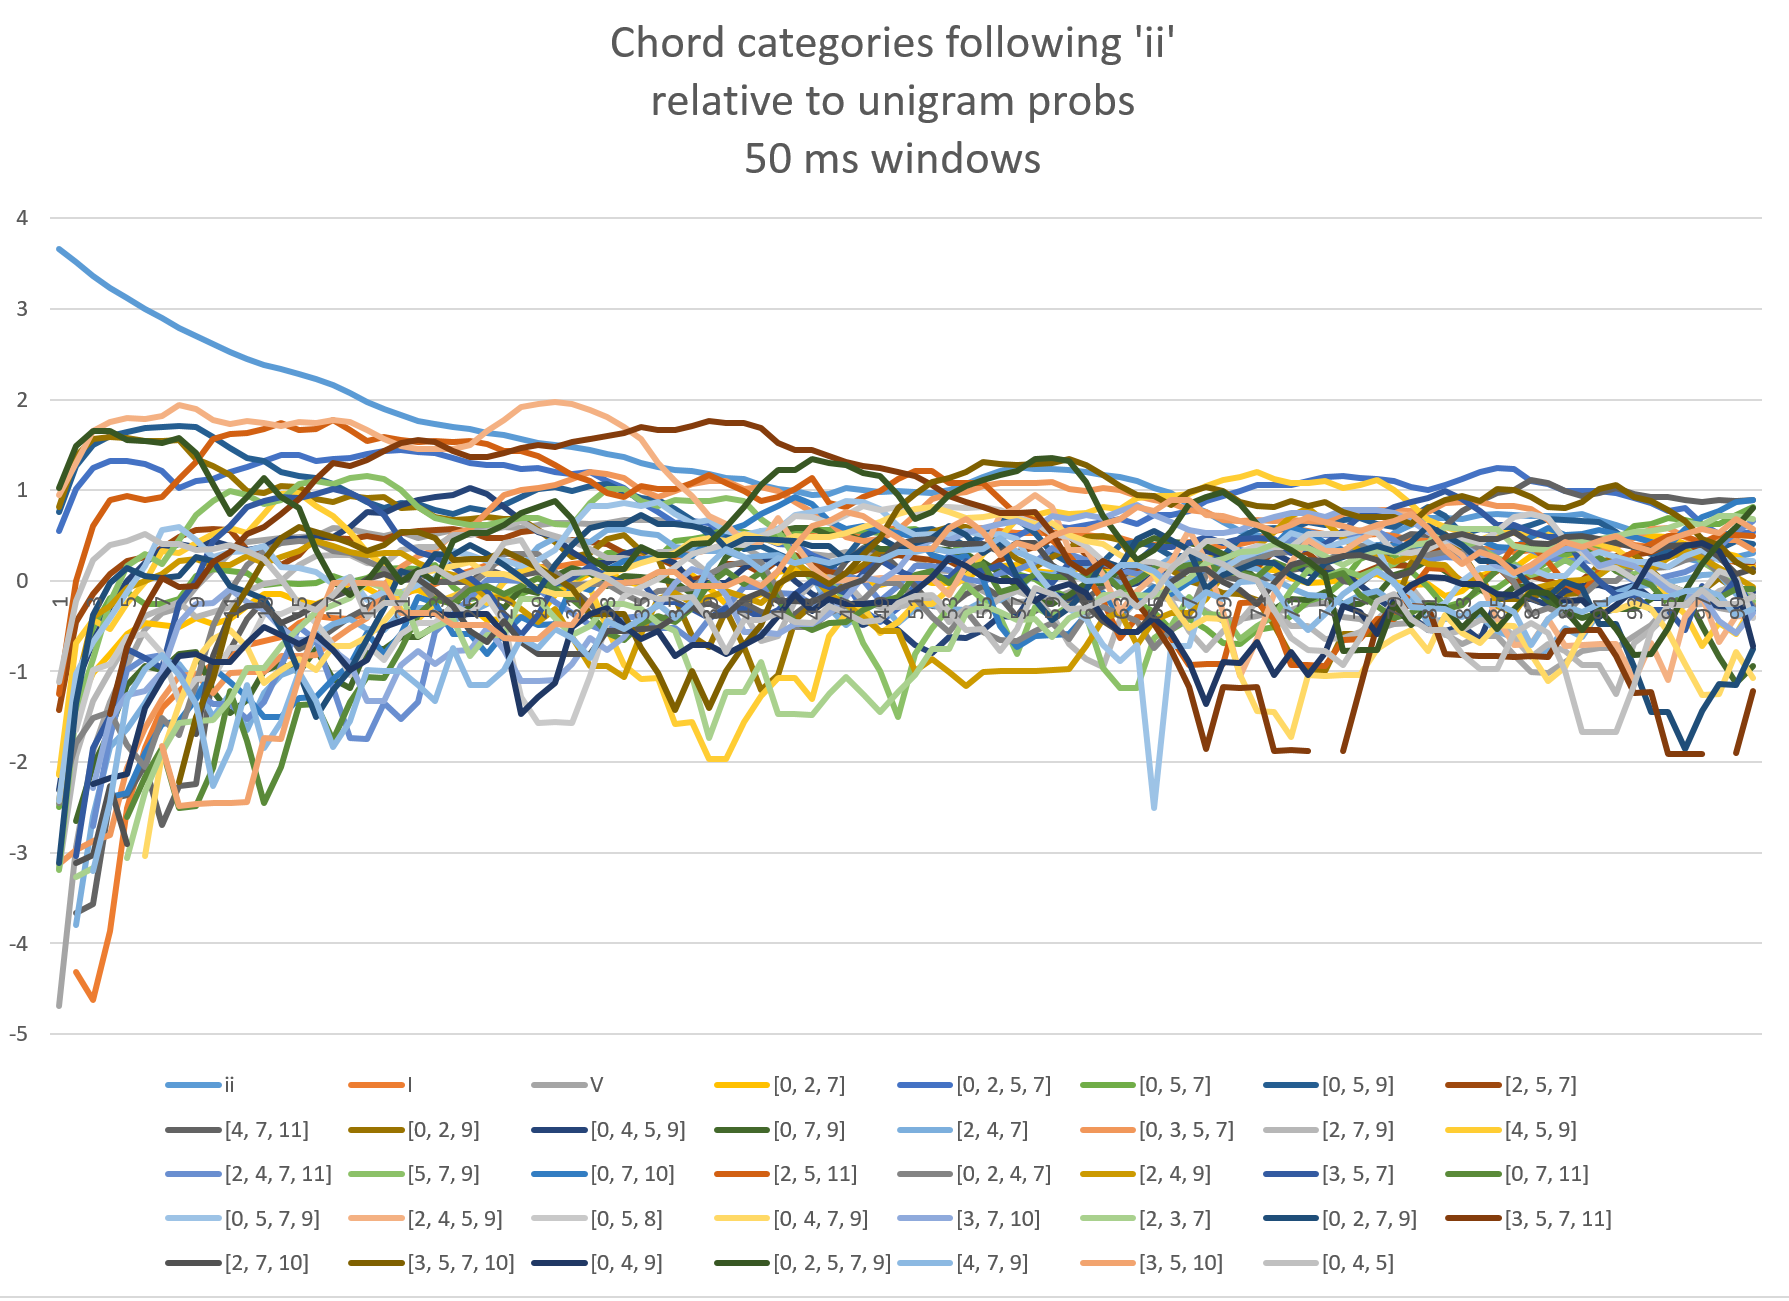
\includegraphics[width=3.5in]{ii_messy.png}
	\end{minipage}
	\begin{minipage}[r]{1.8in}
	{${
	\boldsymbol{\longrightarrow}
	\begin{bmatrix}
		dc_{11} & dc_{12} & dc_{13} & \dots  & dc_{1t} \\
		dc_{21} & dc_{22} & dc_{23} & \dots  & dc_{2t} \\
		dc_{31} & dc_{32} & dc_{33} & \dots  & dc_{3t} \\
		\vdots 	& \vdots  & \vdots  & \ddots & \vdots  \\
		dc_{n1} & dc_{n2} & dc_{n3} & \dots  & dc_{nt}
	\end{bmatrix}
	}$}
	\end{minipage}
\label{plotToMat}
\end{figure}

Associating chord identity with temporal probability distributions invokes a radical kind of behavioralism: to find what kinds of origin chords are similar to one another, computational methods allow us to step away from expectations regarding the pitch similarity of the chords entirely.  As far as the algorithmic work is concerned, the chords could be named with labels like $[0,2,5]$, or $[\hat{1},\hat{2},\hat{4}]$, or $(C,D,F)$, or Lucy, or any other label such that distinct scale degree sets receive distinct names, and the same statistical identity would result.

%Behavioralism (if that's a word) over pitch similarity
Characterizing origin chords entirely in terms of their temporal successors sidesteps a variety of questions regarding what descriptive basis is best.  To determine whether a chord like $[2,7,11]$ behaves more like the upper extension of $iii^7$ or the lower extension of $V^7$, we need not compare the rootedness or pitch set overlap between $[2,7,11]$ and any idealized chord labeled with a roman numeral; instead, we might look for other origin chord types that have temporal probability distributions most similar to those of $[2,7,11]$.  Automated clustering algorithms based on the temporal statistics of chord succession accomplish precisely this task at scale and in an unsupervised manner.  In the YJaMP corpus, the statistics support the claim that the pianists I recorded most often use $[2,7,11]$ in ways similar to other ``tonic-type" chords like $iii^7$, $I^6$, and $vi^7$.

\section{Progression matrix similarity}
%Motivate matrix ordering, truncation, and temporal basis reduction
%too platonic?
Comparing temporal probability distribution matrices requires constructing a consistent metric for quantifying the similarity of any two origin chords.  As the temporal statistics calculated from the YJaMP corpus are finely-grained and sensitive to noise, several steps must be taken to decrease noise and increase the resulting clustering algorithm's chances of discriminating between chords of analytical interest.

%Truncation and ordering
Calculated directly from the corpus, the matrices have differing sizes.  Very uncommon chords which only occur near the end of a few performances might have only a handful of distinct destination chords which ever follow them, producing matrices with only a few rows.  At the other extreme, the most common chords (like tonics) might be followed by more than 1,000 distinct chords across their many appearances in the corpus.  Additionally, some matrices are quite sparse, including nearly-empty rows for many destination chords which only appear once or twice across the entire corpus.  Truncating the size of the tracked chord lexicon and imposing a consistent row ordering across all the resulting origin chord matrices mitigate both problems.

\begin{figure}
	\centering
	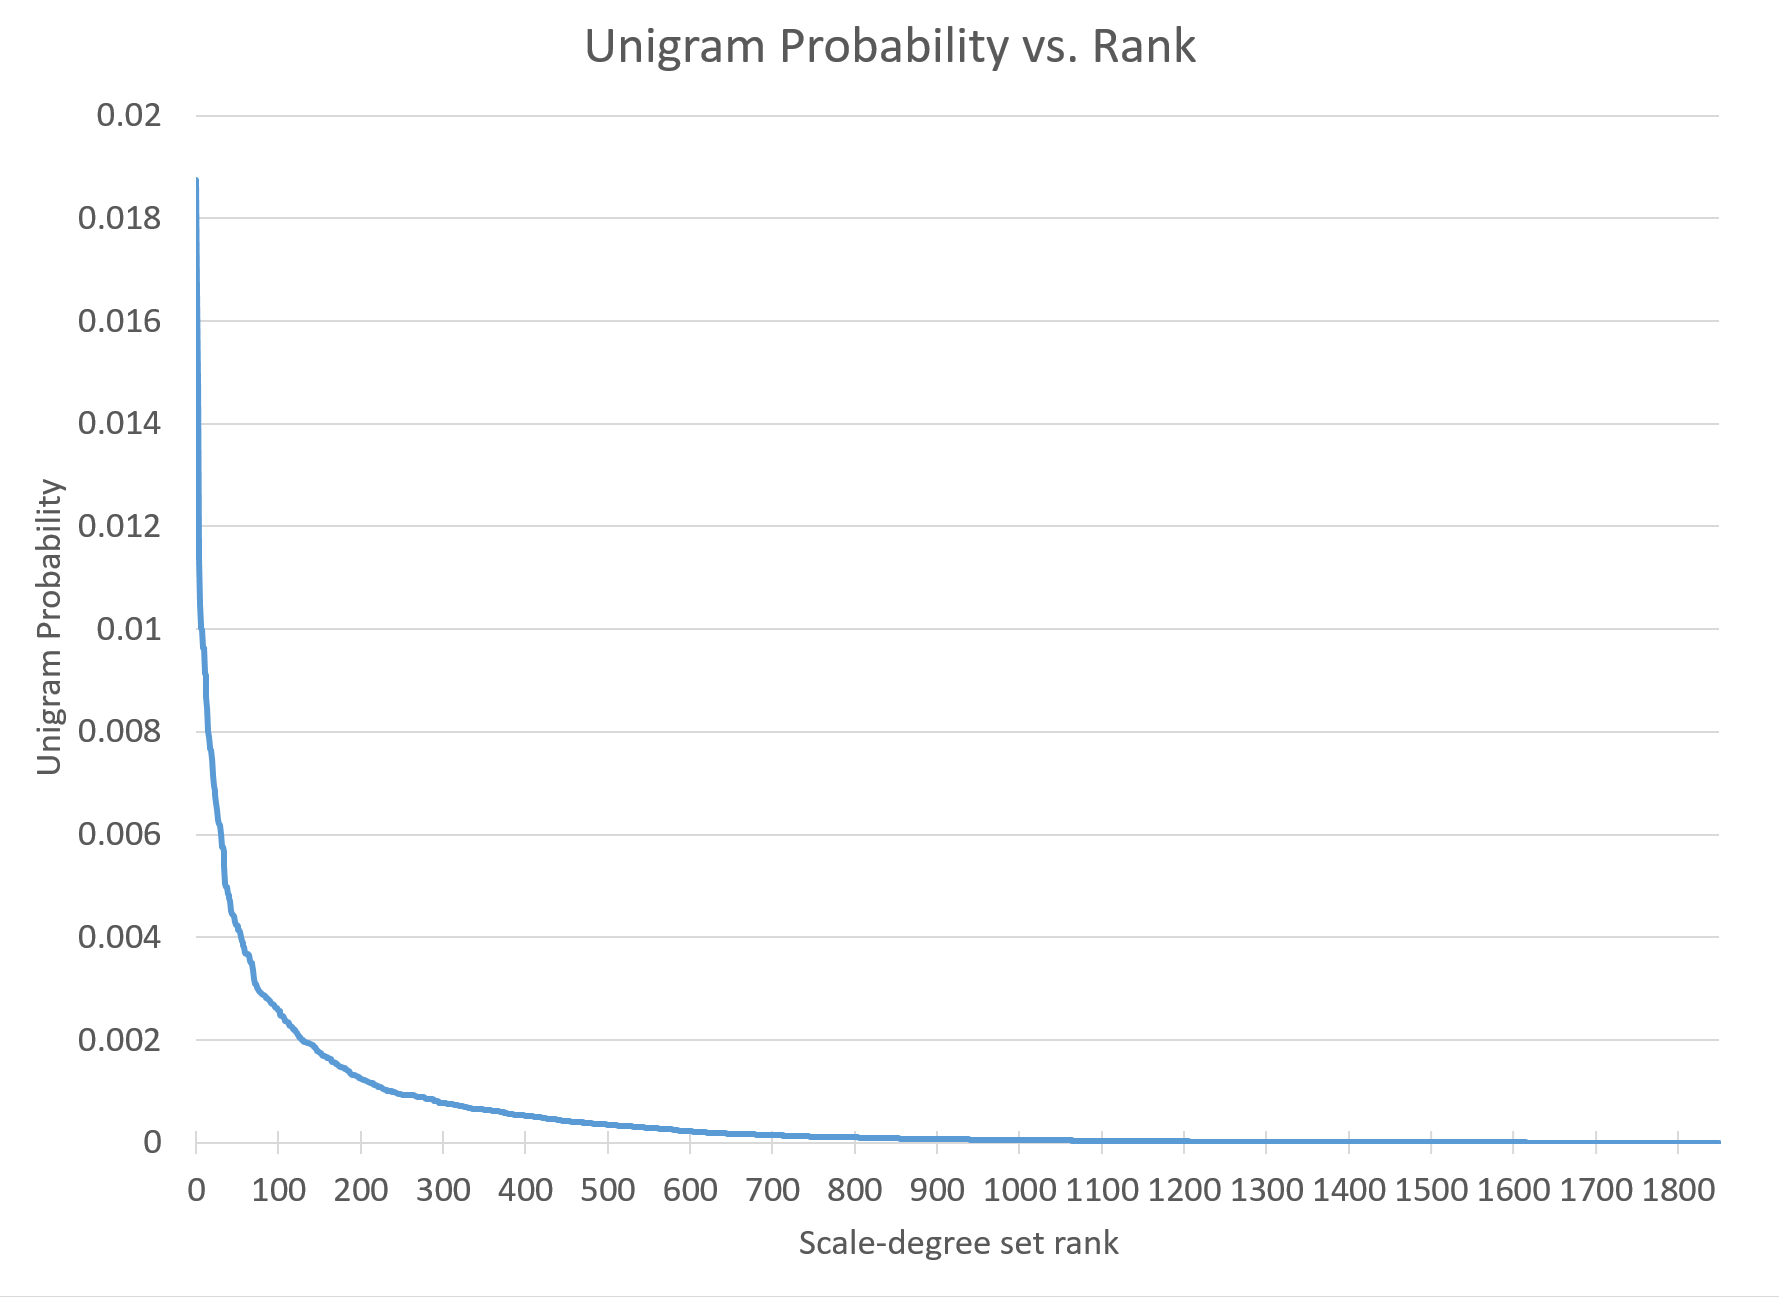
\includegraphics[width=6in]{lexicon_zipfian.png}
	\caption{The unigram probabilities for each of the 1850 distinct scale-degree sets of cardinality three or greater in the YJaMP corpus.  The scale-degree sets are ordered by descending unigram probability.  After around 200 scale-degree sets, the share of overall unigram probability captured by each new marginal set falls below $0.1\%$.}
	\label{lexicon}
\end{figure}

%Truncation and Zipf
Figure~\ref{lexicon} shows the overall unigram distribution for each of the 1850 distinct scale-degree sets of cardinality three or greater.  Like the unigram corpora of many language-like formal systems, it bears resemblance to a Zipfian distribution, where the unigram probability is inversely proportional to each chord's unigram frequency rank.\footnote{Cite some generic Zipf linguistic studies.}  For YJaMP, the distribution of Figure~\ref{lexicon} actually slopes off more slowly than a true Zipf distribution, with the leftmost part of the curve resembling $\frac{1}{r^s}$ for $0.5 < s < 1$.  For quasi-Zipfian distributions, it is common to truncate the size of the lexicon at some rank indicative of diminishing marginal probability gain. For a na\"{i}ve model consisting of only the most probable chord in the corpus -- that is, a model which guesses that every chord observed ought to be the most common chord in the corpus -- adding a second chord to the model nearly doubles the portion of the corpus data it captures.  Instead of describing the observed chord correctly only 2\% of the time, the model can now describe nearly 4\% of the observations in the corpus.  For a 200 chord model, adding one additional chord only captures at most an additional $0.1\%$.  I deem such an increase in model accuracy unworthy of the substantial increase in complexity.\footnote{Zipfian studies (and corpus-driven models in general) spend considerable time fighting over whether or not given distributions contain ``elbows," where a clear change in the first derivative of the curve signals a justifiable alphabet truncation size.  YJaMP's unigram distribution provides no obvious elbow, but the choice of precise alphabet size is a low-stakes game; choosing a number of chords slightly below or somewhat above 200 changes the model's ultimate category assignments by a small amount, and other alphabet size choices are defensible.}

%point out that lexical truncation is a kind of reduction
For computational models, this truncation resembles a statistical analog to traditional music theoretical  voice-leading reduction, though with a narrowly defined justification.  While a human analyst might discount a particular sonority as arising from voice-leading embellishment, lexical truncation discounts only chords with infrequent appearance in the corpus, regardless of the context in which they appear.  The statistics and category assignments resulting from the truncated lexicon may later guide analytical decisions regarding the discarded sonorities, but the outcasts are formally excluded from the model's representation scheme.  Bias creeps into the data here, but in a way that seems most productive for the aims of the model.\footnote{Computational alphabet-size reduction schemes vary in their subtlety, ranging from mere probability truncations like this to sophisticated encodings of human-analytical intuitions; for a good example of the latter, see White 2013.}

%Manhattan metric and PCA justification
With a 200-chord lexical restriction in place, each origin chord can then be associated with an identically-sized 200 by 100 matrix; the 200 rows correspond to the destination chord probability distributions for the 200 most frequent chords in the corpus, in rank order, and the 100 columns correspond to 100 consecutive 50-millisecond time windows.  For the sake of consistency, ``empty rows" (consisting entirely of zeroes) appear for destination chords which never follow a given origin chord within five seconds.  Identically-sized matrices can be compared element-by-element, dramatically simplifying the construction of similarity metrics.\footnote{There are two main streams of machine learning based on matrices (formally, two-dimensional tensors) of this kind; the simplest (introduced here) essentially vectorizes each matrix, flattening its elements to calculate distances via simple dot products.  Tensor learning, on the other hand, retains the structure of each matrix, though implementation of tensor learning is more difficult than vector cases.}  The Manhattan (or ``Taxicab") distance, a special case of the Minkowski distance metric, sums the difference between corresponding entries in two vectors or flattened arrays.  For vectors $x$ and $y$ with $n$ dimensions each, the Manhattan distance $d_1$ is given by
\begin{eqnarray*}
x &=& (x_1,x_2,...,x_n) \\
y &=& (y_1,y_2,...,y_n) \\
d_1(x,y) &=& \sum_{i=1}^n \lvert x_i - y_i \rvert
\end{eqnarray*}
The ``Manhattan" and ``Taxicab" monikers arise from a common geometric interpretation of this distance: for the case of two-dimensional vectors $x$ and $y$, the metric is exactly analogous to the distance traveled by a taxicab between any two points on the square-block grid of Manhattan.  If no diagonal avenues are allowed, a taxi can only travel along roads which intersect at right angles.  Accordingly, the driving distance between any two points on the grid can be calculated from the sum of the east-west blocks and north-south blocks separating the origin and destination points.  The Manhattan metric is easily adapted to the matrix comparison task at hand -- each destination chord probability distribution is a 100-dimensional vector, and the Manhattan distance between two such vectors is the sum of the differences between each of their corresponding elements.  If each destination chord vector were viewed as the coordinates of a point in a 100-dimensional geometric space, the resulting Manhattan distance would be the number of ``blocks" traveled by a taxicab moving in one dimension at a time from one point to another.

A na\"{i}ve, element-by-element Manhattan comparison between two temporal probability distribution matrices, however, implies an identical weighting for probability differences in each time window.  While the predictive and functional properties of chords presumably diminish over time, the contributions of background noise and random variation between destination chord distributions will not.  Consider a limiting case, where the temporal probability distributions for destination chords are 1,000-dimensional vectors tracking the appearance of destination chords as late as 50 seconds after a given origin chord.  At times far after an origin chord, the destination chord distributions will almost certainly reflect the background unigram probabilities plus a contribution from small, random fluctuations uncorrelated to a particular origin chord or category.  A Manhattan metric applied to vectors in this high-dimensional space will tally increasing contributions from the random fluctuations, proportionally, drowning out the patterns in phonetic or syntactic progressions at shorter time scales.

%PCA saves the day
Just as it did in Chapter 3, PCA allows the extraction of time scales over which chord distributions experience the highest variance with few assumptions regarding which time scales are too short or too long.  Each origin chord is associated with a matrix of destination chords, and each destination chord is represented by a row of 100 coordinates, each of which indicates the probability of the destination chord's appearance a given number of time windows after the origin chord.  But these 100 coordinates are not the only way to represent the destination chord's probability variance over time.  For each origin chord, running PCA on the set of 100-dimensional destination chord distributions produces a set of principal components, 100-dimensional vectors themselves, capturing the combinations of time windows which account for the greatest amount of variance in the destination chord distributions.  In a way, (combinations of) the principal components provide ready-made templates designed to capture the most common temporal differences between kinds of destination chord behavior.  Destination chord probability distributions can then be written with a much smaller number of coordinates while losing as little accuracy as possible.  Instead of using coordinates to say ``This destination chord appears with 10\% probability at $t=1$, and 5\% probability at $t=2$, and ...", the new coordinate system might be translated to say ``This destination chord's probability curve looks like $1.2$ times the curve given by the first principal component, plus $2$ times the curve given by the second component, plus..."

In this way, each destination chord probability distribution -- each row of the origin chord's associated temporal matrix -- undergoes a basis transformation, a change in its method of coordinate description.  As described in Chapter 3, a PCA algorithm calculates the components themselves by examining coordinate variance across the full set of destination chords of a given matrix, providing one optimized set of principal components per origin chord with which to re-describe them.  And for most origin chords, especially those with high unigram probabilities, the PCA components resemble the phonetic, syntactic, and background components found for $ii$'s destination chords in Chapter 3.

Figure~\ref{PCA_examples} shows four sets of principal components capturing most of the variance in destination chord temporal probability distributions for four different origin chords.  In each case, I have retained the first three principal components.  For nearly all of the 200 most probable chords, three components are enough to capture at least 75\% of the variance in destination chord distributions; in many cases, three components capture more than 90\%.  In each plot of Figure~\ref{PCA_examples}, the components are color-coded in order of descending variance capture: the first component is blue, and typically captures more than 50\% of the variance, while the second and third components are green and red, respectively.  The horizontal axis tracks 50ms time windows, while the vertical axis indicates each component's probability loading per time window.  If an origin chord matrix contained a destination chord with a probability distribution that happened to look exactly like the first principal component, that distribution could be described in this new basis with the coordinates $(1,0,0)$ -- one multiple of the first component, and no contributions from either other component distribution.

%figure: PCA components for 4 top-200 origin chords to explain temporal basis reduction and component alignment
\begin{figure}
	\centering
	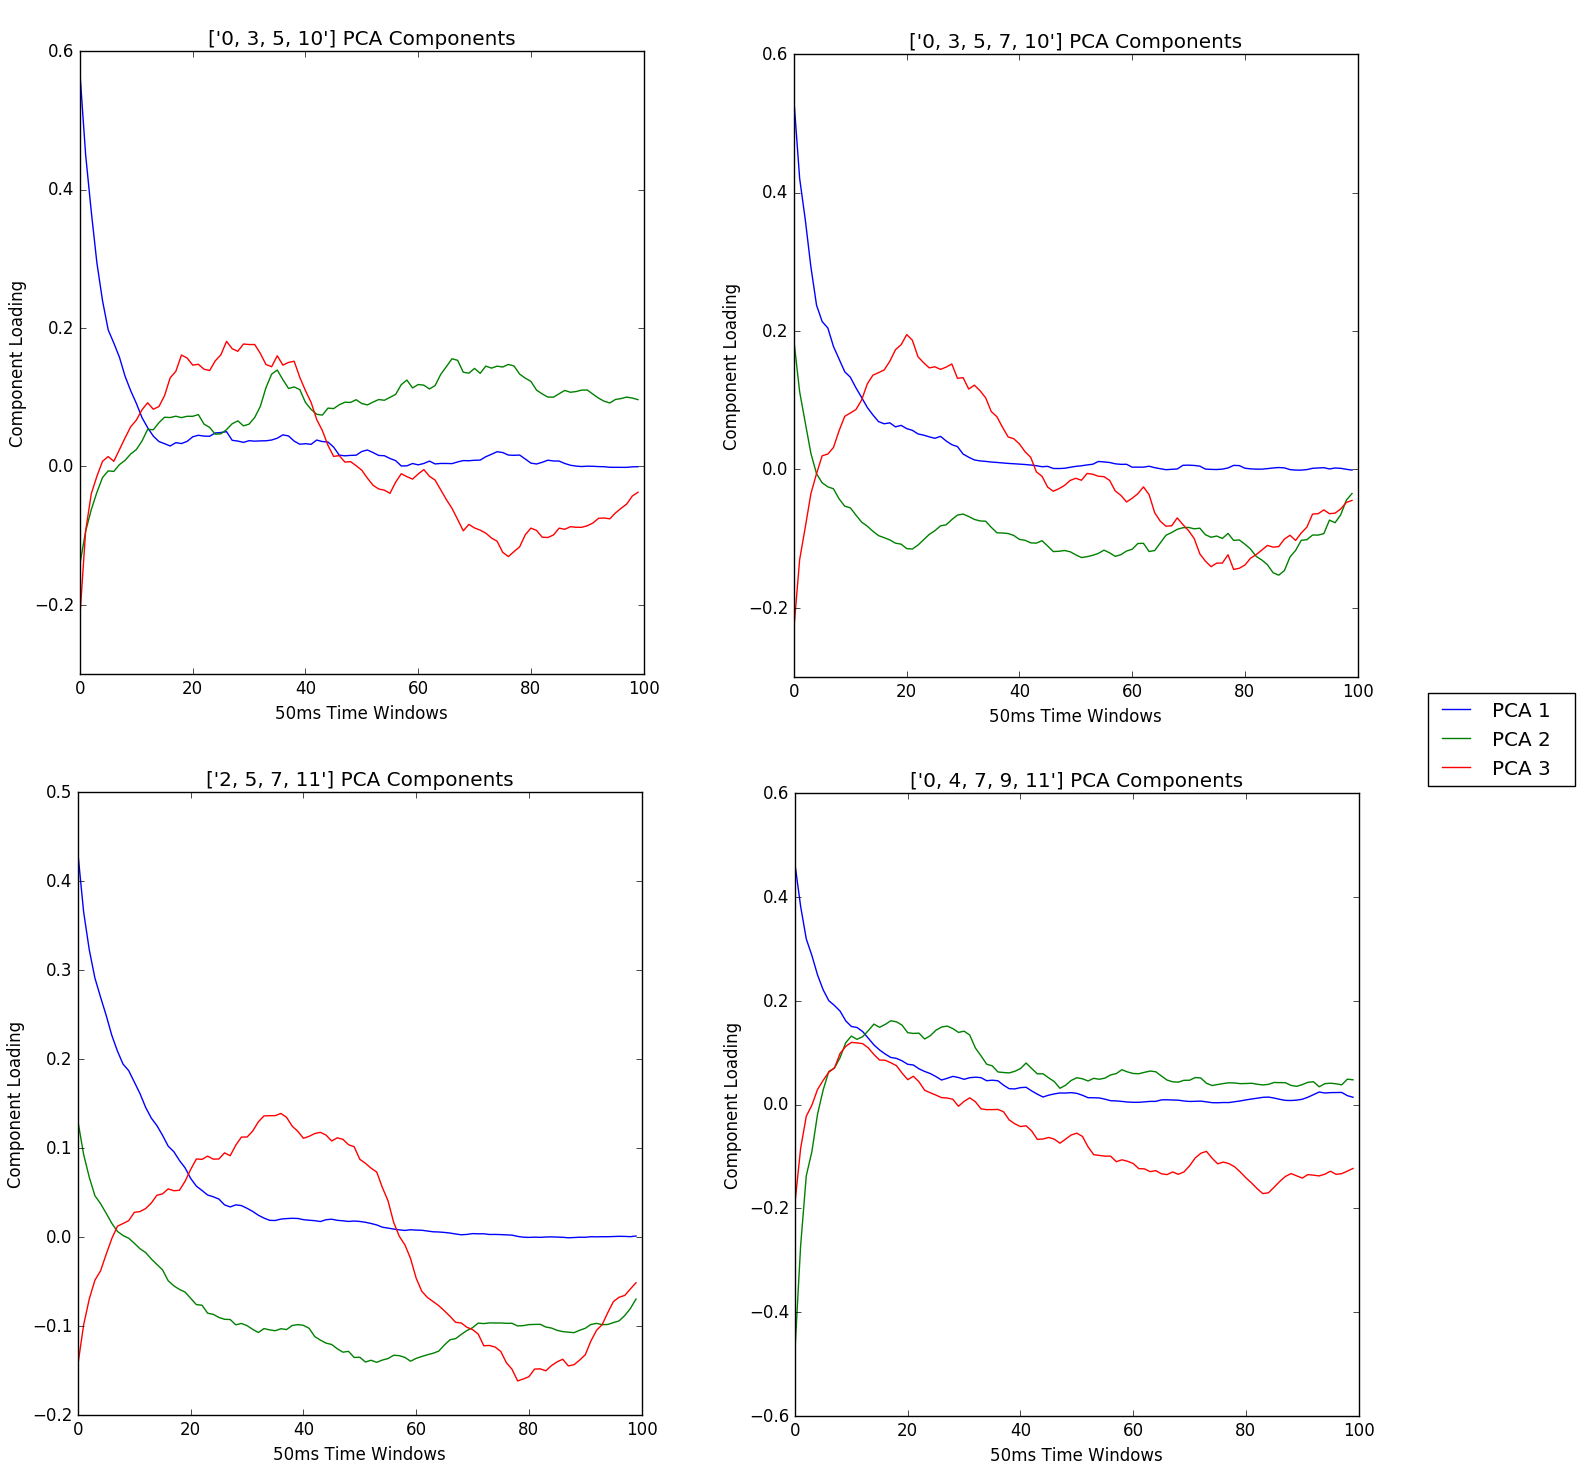
\includegraphics[width=6in]{top200_PCA.png}
	\caption{The first three principal components capturing the most temporal probability variance for four selected origin chords.  For each origin chord, the components provide a three-dimensional reduction of the 100-dimensional destination chord distributions.  Each destination chord's temporal probability distribution can then be written with only three coordinates -- the loadings for each principal component.}
	\label{PCA_examples}
\end{figure}

The top left plot in Figure~\ref{PCA_examples}, calculated from the origin chord $[0,3,5,10]$, shows principal components which directly correspond to the intuitions developed in Chapter 3 regarding temporal progression regimes.  The first (blue) component correlates high initial probability variance shortly after the origin chord with a decrease in variance over time; high coordinate values along this component capture chord behavior characteristic of the phonetic temporal regime, in which origin chords tend to progress to voice-leading neighbor destination chords with similar traditional harmonic functions over short time scales.  Compared to a randomly-chosen destination chord, a phonetic neighbor with a high PCA component 1 score would likely display a large deviation from unigram probability at short time scales, and the deviation in probability would trail off as time after the origin chord increases.  The second (green) component correlates initial probability suppression with a gradual ascent to a stable, non-zero probability value at later times, a combination well-suited to the probabilistic variance of chords common to the local key context but comparatively unlikely to occur as voice-leading neighbors to $[0,3,5,10]$.  The more complex third (red) component implies the most subtle type of temporal progression, yielding a template for destination chords which are suppressed during the phonetic regime but have higher probabilities during a finite time span afterward.  I suggested in the previous chapter that this kind of behavior captures a possible translation of ``syntactic progressions," in traditional theory parlance, where chords unlikely to serve the same local function as the origin chord are more highly probable shortly thereafter than in the long term.  Combinations of these components render the status of many destination chords ambiguous, but this simplified explanation serves to indicate the connection between principal components and destination chord probability distributions in broad strokes.

The components for the other origin chords of Figure~\ref{PCA_examples} serve to block over-interpretation of the salient features of $[0,3,5,10]$.  In each case, component one matches phonetic-scale probability expectations, but one or both of the other components appear quite different.  The nature of this difference arises from PCA itself.  If each component provides a new basis direction along which destination chords are likely to show great variance, the orientation of any particular destination chord's variance along that direction is not reflected in the principal component.  Each component captures not just one kind of probabilistic behavior, but \emph{two}: if a destination chord distribution exactly resembling the first component can be assigned PCA-basis coordinates $(1,0,0)$, a destination chord distribution showing exactly the opposite behavior -- strongly suppressed at short distances, asymptotically increasing over long durations -- could be captured by the coordinates $(-1,0,0)$.  The same component would exactly capture the probability fluctuations of the destination chord, but the relevant coordinate would carry a negative sign.

Figure~\ref{PCA_examples} thus serves as an encoded set of instructions for how to find particular kinds of chords.  To find destination chords after $[0,3,5,10]$ matching intuitive expectations for phonetic, background, and syntactic-regime progressions, the analyst should examine chords with high, positive coordinate scores along each of the three principal components.  For $[0,3,5,7,10]$, the PCA components for which appear in the top right portion of Figure~\ref{PCA_examples}, the same is true up to a correction of sign: destination chords with phonetic and syntactic regime behavior will be written with high, positive coordinates along PCA components one and three, but background-type destination chords will be written with \emph{negative} scores along the direction of PCA component two.  In other words, component two for $[0,3,5,7,10]$ resembles the mirror image of component two for $[0,3,5,10]$, its multiple by negative one, so background destination chords with positive coordinates along component two for $[0,3,5,10]$ will have similar probability distributions to destination chords with negative components along component two for $[0,3,5,7,10]$.  The same sign change describes the component difference for the bottom-left plot of Figure~\ref{PCA_examples}, $[2,5,7,11]$; like $[0,3,5,7,10]$, its second component resembles the mirror image (or negative multiple) of the second component of $[0,3,5,10]$.

The easiest way to attempt to clarify interpretations of the principal components is to check how common chords are represented in the new basis.  For the bottom-left case on Figure~\ref{PCA_examples}, $[2,5,7,11]$, we can check which destination chords have the largest component loadings -- the biggest coordinates in each dimension of the new basis -- to see if they correlate with temporal progression regime interpretations.  In this test case, the chords with highest component one loadings are $[2,5,7,11]$, $[5,7,11]$, $[2,7,11]$, and $[2,5,7]$, all scale-degree sets we might expect to show up in the phonetic regime, as they all resemble objects often characterized as incomplete voicings of $V^7$ chords.  Generalizing that observation, we might expect to find voice-leading neighbors and other phonetic-scale progressions automatically by extracting destination chords with large component one coordinate values.  The PCA algorithm does not know that these chords share a traditional functional interpretation or that they have pitches in common; it only knows that they tend to appear in close temporal proximity to one another.

To check if the second principal component for $[2,5,7,11]$ maps onto syntactically-suppressed progressions, we can look for the destination chords with largest \emph{negative} component two loadings.  The top four are $[4,7,11]$, $[2,5,9]$, $[2,3,7]$, and $[0,2,5]$.  Two of these destination chords are recognizable $ii$ or $ii^7$ scale-degree sets ($[2,5,9],[0,2,5]$), which should appear frequently in tonal progressions but \emph{not} immediately after a $[2,5,7,11]$ chord.  Scale-degree sets resembling $iii$ and $\flat III^7$ also appear here, and their status is less clear.  The latter may reflect major-minor key ambiguities  (since a minor key featuring $i$ and $V$ may well feature progressions involving the relative major, $\flat III$), while the former may indicate the major-mode tendency for $iii$ to function as a local tonic.  Its initial suppression after $[2,5,7,11]$ would then indicate that $iii$ is not typically approached from this origin chord.

The component three loadings for $[2,5,7,11]$ serve as a cautionary tale for the interpretation of PCA reductions.  Examining purely the highest or lowest values for the component three score does not yield a stable category of any particular kind of progression behavior: most of the scale-degree sets which have the highest and lowest component three values also have high or low scores along the direction of component two.  The largest negative component three score belongs to $[2,3,7]$, while $[4,7,11]$ has the largest positive score.  Since both of these chords have strongly negative component two scores, component three serves to distinguish their progression behavior from one another.  Adding up contributions from components two and three amounts to summing their loading curves, so $[2,3,7]$ will appear with increased probability later after $[2,5,7,11]$ than $[4,7,11]$ will.%This is pretty weak.

The bottom-right plot, $[0,4,7,9,11]$, displays components with similar contours to the other three plots, but on a compressed time-scale.  The rate of decrease in component one and initial increases for components two and three occur much closer to the origin chord than the corresponding components for the other plotted origin chords.  This likely reflects the decreased predictive power of a tonic chord over time.  Within a few time windows after the appearance of $[0,4,7,9,11]$, component one indicates that voice-leading neighbors still occur with greatly increased probability, but the overall probability variance after 20 windows or so is quite small.  This provides a graphical translation and confirmation of received harmonic wisdom: the appearance of a $I$ or $vi$ chord in a any particular key tells the analyst very little about what chords likely appear in the future, as nearly any key-appropriate chord can follow tonic chords in a syntactic phrase.

The principal components for a large number of the top 200 most probable chords in the YJaMP corpus afford observations of this nature to such an extent that the comparison of basis components between origin chords can be standardized and automated.  To see if a destination chord shows the same kind of probability fluctuations after two different origin chords, an algorithm can compare the destination chord's PCA-basis coordinates with respect to both origin chords up to an overall alignment of signs.  A metric comparing two origin chords needs only to align the corresponding PCA components by multiplying one or more columns of their basis-transformed destination chord probability matrices by negative one to achieve an imposed, standard alignment: component one starts with positive value at $t=0$, and components two and three start with negative values.  This alignment is arbitrary, and the interpretation of individual components in isolation is often misleading -- but the resulting standardization comes at no real cost and permits similarity comparisons across the set of origin chord matrices.

As a result, I compare origin chords by imposing a Manhattan metric on matrices consisting of the destination chord temporal probability distributions for the 200 most probable chords in the corpus written in a systematically-aligned, PCA-reduced basis.  Each origin chord corresponds to a matrix with 200 rows and three columns, and I employ a dissimilarity ``distance" between two origin chords defined as the sum of the absolute differences between corresponding elements in their respective matrices.  In more formal notation, the distance $d$ between chords $\alpha$ and $\beta$ is given by

\begin{equation}
d(\alpha, \beta) = \sum_{i=1}^{200} \sum_{j=1}^3 \lvert \alpha_{ij} - \beta_{ij} \rvert
\end{equation}

This distance metric remains agnostic about the pitch structures of the origin and destination chords, and it provides a (dis)similarity metric based purely on progression statistics; a larger Manhattan distance $d$ between two matrices $\alpha$ and $\beta$ correlates with a sense of increased difference between the progression behavior of the corresponding origin chords.\footnote{Other metrics imposed on this basis could provide similar results -- especially other Minkowski distances of low order.  The astute reader may notice that this choice of metric discounts much of the 2D tensor structure inherent in the temporal progression matrices; this will return later in the chapter.} As the next section will show, a metric of this kind allows clustering algorithms to group origin chords together based on similarity in their overall progression tendencies, yielding a rough approximation of chord categories assembled from behavioral statistics.

\section{Syntax clustering}
%with Manhattan metric in hand, explain at least flat agglomerative clustering for (functional?) categories
%go into detail about agglomerative hierarchical clustering on the topN-filtered, PCA-transformed matrices
Clustering algorithms, in their simplest form, pursue a single goal: given an array of objects described in some coordinate basis, group the objects into categories where the members of each category are ``closer" (or ``more similar") to one another than they are to members of the other categories.  Aside from the input objects, described with some consistent representation scheme, most clustering algorithms require the analyst to supply two further input choices -- a similarity metric for comparing objects to one another, and a way to determine the boundaries of each cluster.  If the input objects are represented in a basis that lends itself to a geometric interpretation (like spatial coordinates), the process of drawing these cluster boundaries may be interpreted as outlining shapes or surfaces containing the objects.  The resulting points in each category would be found close to one another, geometrically speaking -- ``clustered" together.

%hierarchical clustering in general; greedy algorithms
Hierarchical clustering algorithms approach the very complex problem of how to partition a large number of data points into clusters by splitting it into a series of simpler problems.\footnote{Hierarchical clustering techniques date back to at least Ward 1963, which explicitly generalizes from single-variable clustering problems to efficient strategies for hierarchical groupings of high-dimensional data.}  Starting from either of two limiting cases -- either there is only one giant cluster, into which all data points fall, or every point is its own cluster -- hierarchical clustering first either splits the giant cluster into two smaller clusters (the former, ``divisive" clustering case) or merges an individual point cluster with its closest metric-determined neighbor (the latter, ``agglomerative"  method).  As a result, the algorithm replaces the na\"{i}ve limiting case with a slightly more nuanced approximate clustering.  Repeating the split or merge step many times, hierarchical clustering gradually produces an approximation of the optimal clustering.  For each step, hierarchical clustering algorithms perform what computer scientists refer to as ``greedy" optimization, using all available (dis)similarity information provided by the metric to make the best possible local decision without any consideration of its future effects.  Common implementations of hierarchical clustering make no attempt to guess in advance what cluster assignments many successive splits/merges will produce.  Due to their computationally efficient short-sightedness, such greedy hierarchical clustering algorithms can occasionally get off track, producing final clusterings which poorly capture the intuitive structure of the data.\footnote{See, for example, Berkhin's discussion on pp. 29-36 of Kogan, Nicholas, and Teboulle (Eds.) 2006.}

%bad results from divisive clustering?  Agglom works well; explain it
With no method for planning the end results of the greedy optimization, divisive hierarchical clustering algorithms start with a trickier task than agglomerative ones: there are many possible ways to split a large data set into two clusters, and the immediate differences between initial splits may be small.  For a noisy data set, however, many initially-productive splittings can turn out to produce ill effects in the final clustering, as data points comparatively close together might be placed into different clusters early on to optimize cluster-level criteria.  Agglomerative hierarchical clustering approaches the problem from the opposite direction.  If divisive clustering is a ``top-down" process, requiring a heuristic for how to split clusters most effectively, agglomerative clustering is a ``bottom-up" procedure, where each merge step uses the metric to determine which points (or groups of points) are closest together.  Closely-related objects are less likely to end up placed far apart, but another kind of judgment call is still required: a linkage criterion indicating how to calculate the distance between a single data point and a cluster of arbitrary size.  If a merge operation places a point (or many points) into a cluster, it must evaluate which cluster would be the best, ``closest" assignment.  Several ways of specifying this linkage criterion are possible, but ``complete" or ``maximum" linkage provides the best results for clustering the YJaMP temporal probability matrices.\footnote{Two types of sub-optimal behavior accrue as a result of other linkage criteria: either category assignments violate a large number of syntactic expectations, or the resulting clusters differ radically in size -- one cluster might have 100 origin chords, and a dozen other clusters might contain a handful of chords each.  This human-heuristic validation of model criteria implicates a complex network of algorithm-analyst interaction, some features of which will appear in \S 4.5 below.}

Maximum linkage defines inter-cluster distance to be the \emph{largest} distance between any two points in the respective clusters.  Put formally, the distance ($d_l$) between two chord clusters $A$ and $B$ can be calculated from the Manhattan-metric distances ($d_m$) between the chords in each cluster:
\begin{equation}
\label{eq:d_l}
d_l(A,B) = \max \{ d_m(c_1,c_2) \vert c_1 \in A, c_2 \in B \}
\end{equation}
Each merge step adds a single point to a cluster or combines two clusters in order to optimize the linkage criterion $d_l$.  After many such merge steps, agglomerative hierarchical clustering produces cluster assignments for the full range of observations -- in YJaMP's case, the top 200 most probable origin chords.

%now describe the results
%First, what the dendrogram even means
Running agglomerative hierarchical clustering of this kind with the sklearn (``scikit-learn") Python package produces the dendrogram given in Figure~\ref{Dend_complete}.  The 200 most unigram-probable chords are listed at the bottom of the figure in an order automatically chosen to keep cluster members adjacent to their nearest neighbors.  Each bracket on the dendrogram represents a merge operation, and the vertical-axis height of each bracket reflects the distance between its two associated ``children."  At the bottom of the figure, origin chords connected by a bracket constitute merges which associate a single chord (or ``leaf," in dendrogram parlance) with the chord deemed most similar to it -- that is, with the chord which minimizes $d_l$ in Equation~\ref{eq:d_l} above.  Higher up in the ``tree," branchings indicate merge steps where at least one of the clusters contains multiple chords.  Hierarchical clustering provides multiple levels of similarity ranging from point-to-point up to broad cluster-to-cluster comparisons.  In YJaMP's terms, this range of groupings indexes both similarity between individual chords (near the bottom of the tree) and a functional or modal organization of the origin chords into a small number of categories (near the top of the tree).

The color coded portion of the tree in Figure~\ref{Dend_complete} provides rough category assignments for the clusters.  The decision where to ``cut" the dendrogram into large-scale category clusters is comparatively arbitrary, and I impose it here via the Python package SciPy's \emph{fcluster} function, which color codes clusters based on a supplied inter-cluster distance, a particular choice of vertical-axis height at which to identify categories.  I set that threshold high enough reduce the number of clusters as much as possible while minimizing the extent to which clusters containing functionally-different chords are merged.  As this is a heuristic decision, other choices of cut point are clearly defensible, and imposing them merely requires modifying the color-coding on Figure~\ref{Dend_complete}, choosing instead to categorize clusters at a slightly higher or lower location on the dendrogram.  As it stands, Figure~\ref{Dend_complete} color codes 59 potential clusters, 28 of which contain more than one chord.  Table~\ref{memb} provides a list of the scale-degree sets assigned to each (arbitrary) cluster label.  The full dendrogram is difficult to read, so a series of subplots appear below.

%the big agglom clus dendrogram, at least three subplots thereof with annotation and explanation
\begin{landscape}
\begin{figure}
	\centering
	\caption{The full dendrogram for agglomerative hierarchical clustering of the top 200 most frequent chords in the YJaMP corpus.  Chord-to-chord distances (or dissimilarities) are calculated from PCA-reduced temporal probability distribution matrices for each chord.}
	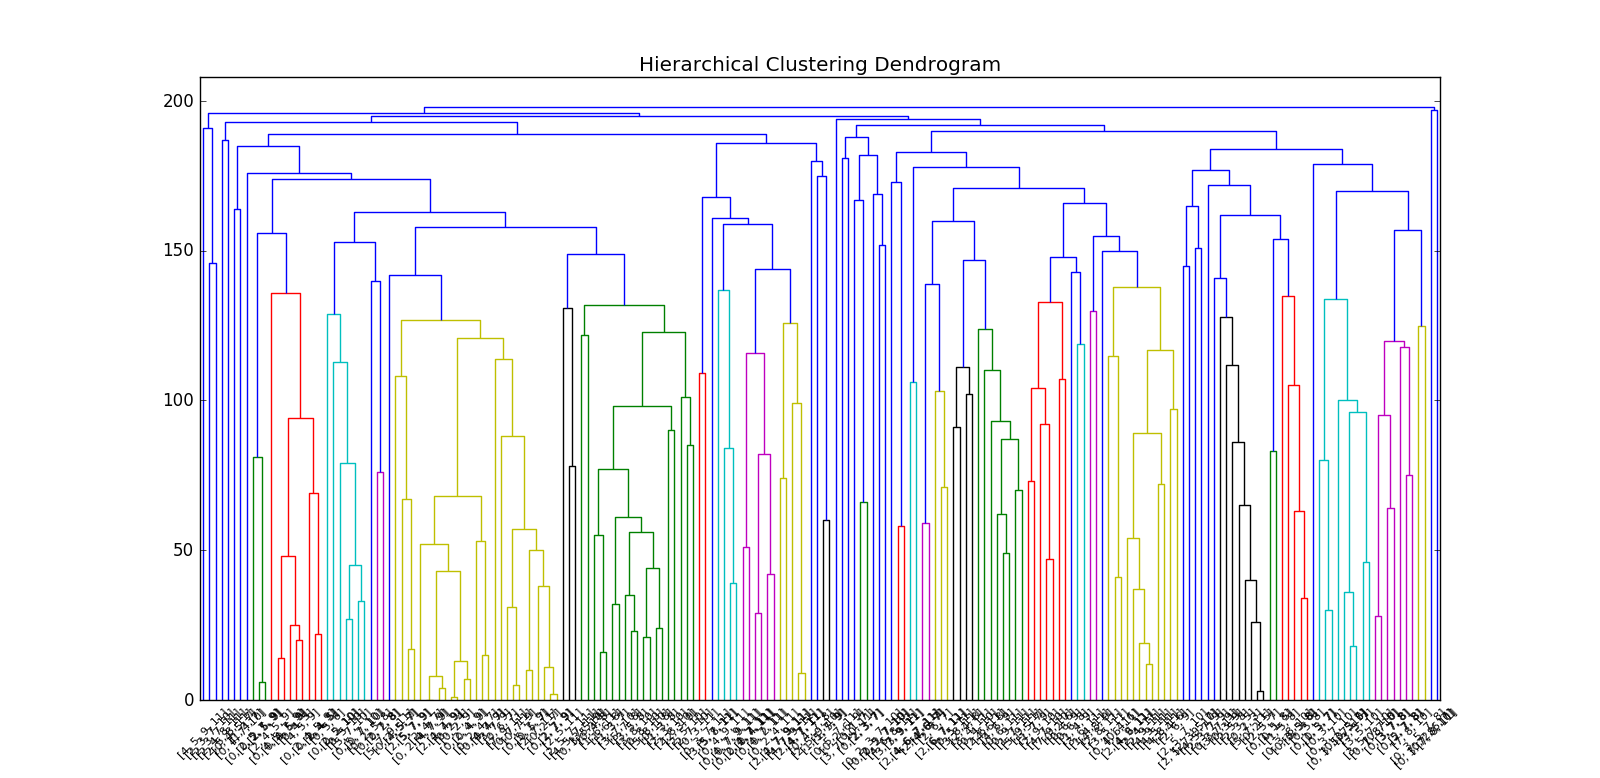
\includegraphics[width=9in]{Dendrogram_complete.png}
	\label{Dend_complete}
\end{figure}
\end{landscape}

%\begin{landscape}
\begin{table}
	%\centering
	\caption{The 200 most unigram-probable scale-degree sets in the YJaMP corpus grouped into clusters via flattened agglomerative clustering.  The cluster label numbers are arbitrary, except to indicate adjacency.}
	\label{memb}
\begin{multicols}{3}
{\small
\begin{tabular}[t]{r |l }
\hline\hline
cluster & scale-degree set\\ [0.5ex]
\hline
1	&	[2, 3, 7, 10]	\\
2	&	[2, 3, 7, 11]	\\
3	&	[4, 5, 9, 11]	\\
4	&	[2, 4, 8, 11]	\\
5	&	[2, 5, 8, 11]	\\
6	&	[0, 4, 5, 7]	\\
7	&	[0, 4, 7, 10]	\\
8	&	[0, 2, 5, 7, 9]	\\
	&	[0, 2, 5, 9]	\\
	&	[2, 5, 9]	\\
9	&	[0, 2, 4, 5, 9]	\\
	&	[0, 2, 4, 5]	\\
	&	[0, 4, 5, 7, 9]	\\
	&	[0, 4, 5, 9]	\\
	&	[0, 4, 5]	\\
	&	[0, 5, 9]	\\
	&	[2, 4, 5, 9]	\\
	&	[2, 4, 5]	\\
	&	[4, 5, 9]	\\
10	&	[0, 2, 10]	\\
	&	[0, 2, 5, 10]	\\
	&	[0, 5, 10]	\\
	&	[0, 5, 6]	\\
	&	[0, 5, 7, 10]	\\
	&	[0, 7, 10]	\\
	&	[5, 7, 10]	\\
11	&	[0, 2, 5, 8]	\\
	&	[0, 2, 7, 8]	\\
	&	[0, 2, 8]	\\
12	&	[0, 2, 4, 7, 9]	\\
	&	[0, 2, 4, 7]	\\
	&	[0, 2, 4, 9]	\\
	&	[0, 2, 4]	\\
	&	[0, 2, 5, 7]	\\
	&	[0, 2, 7, 9]	\\
	&	[0, 2, 7]	\\
	&	[0, 2, 9]	\\
	&	[0, 4, 7, 9]	\\
	&	[0, 4, 7]	\\
	&	[0, 4, 9]	\\
	&	[0, 5, 7, 9]	\\
	&	[0, 5, 7]	\\
\end{tabular}
\vfill
\columnbreak
\begin{tabular}[t]{r |l }
\hline\hline
cluster & scale-degree set\\ [0.5ex]
\hline
12	&	[0, 6, 7]	\\
	&	[0, 7, 11]	\\
	&	[0, 7, 9]	\\
	&	[2, 4, 7, 9]	\\
	&	[2, 4, 7]	\\
	&	[2, 4, 9]	\\
	&	[2, 5, 7, 9]	\\
	&	[2, 7, 11]	\\
	&	[2, 7, 9]	\\
	&	[3, 7, 9]	\\
	&	[4, 5, 7]	\\
	&	[4, 7, 9]	\\
	&	[5, 7, 9]	\\
	&	[7, 9, 11]	\\
13	&	[5, 7, 9, 11]	\\
14	&	[2, 5, 11]	\\
	&	[2, 5, 7, 11]	\\
	&	[4, 5, 7, 11]	\\
15	&	[0, 1, 8]	\\
	&	[0, 3, 5, 10]	\\
	&	[0, 4, 8]	\\
	&	[0, 8, 10]	\\
	&	[1, 3, 7]	\\
	&	[1, 3, 8]	\\
	&	[1, 6, 11]	\\
	&	[1, 6, 8]	\\
	&	[2, 3, 10]	\\
	&	[2, 3, 9]	\\
	&	[2, 5, 10]	\\
	&	[2, 7, 10]	\\
	&	[2, 8, 10]	\\
	&	[3, 5, 8]	\\
	&	[3, 5, 9]	\\
	&	[3, 7, 10]	\\
	&	[3, 8, 10]	\\
	&	[5, 7, 8]	\\
	&	[5, 8, 10]	\\
16	&	[1, 4, 7]	\\
17	&	[0, 3, 11]	\\
	&	[0, 3, 7, 11]	\\
18	&	[0, 4, 7, 9, 11]	\\
	&	[0, 4, 9, 11]	\\
\end{tabular}
\vfill
\columnbreak
\begin{tabular}[t]{r |l }
\hline\hline
cluster & scale-degree set\\ [0.5ex]
\hline
18	&	[0, 7, 9, 11]	\\
	&	[5, 8, 11]	\\
19	&	[0, 2, 11]	\\
	&	[0, 2, 4, 11]	\\
	&	[0, 2, 4, 7, 11]	\\
	&	[0, 2, 7, 11]	\\
	&	[0, 4, 11]	\\
	&	[0, 4, 7, 11]	\\
20	&	[2, 4, 7, 11]	\\
	&	[2, 4, 7, 9, 11]	\\
	&	[2, 7, 9, 11]	\\
	&	[4, 7, 11]	\\
	&	[4, 7, 9, 11]	\\
21	&	[3, 5, 7, 11]	\\
22	&	[1, 5, 7, 9]	\\
	&	[1, 5, 9]	\\
23	&	[2, 5, 9, 10]	\\
24	&	[0, 4, 7, 8]	\\
25	&	[0, 2, 6, 9]	\\
26	&	[3, 7, 10, 11]	\\
27	&	[0, 2, 3, 7]	\\
	&	[2, 3, 7]	\\
28	&	[0, 1, 7]	\\
29	&	[0, 2, 5, 7, 10]	\\
30	&	[0, 2, 7, 10]	\\
31	&	[0, 2, 3, 7, 10]	\\
32	&	[3, 7, 9, 11]	\\
	&	[3, 9, 11]	\\
33	&	[4, 6, 8, 11]	\\
34	&	[2, 4, 6, 7, 11]	\\
	&	[4, 6, 7, 11]	\\
35	&	[2, 4, 6, 7]	\\
	&	[2, 6, 7, 11]	\\
	&	[2, 6, 7]	\\
	&	[4, 6, 7]	\\
	&	[6, 7, 11]	\\
36	&	[0, 5, 11]	\\
	&	[2, 4, 8]	\\
	&	[3, 4, 11]	\\
	&	[3, 8, 11]	\\
37	&	[0, 4, 10]	\\
	&	[0, 6, 11]	\\
\end{tabular}
}
\vfill
\end{multicols}
\end{table}

\begin{table*}
\caption*{(Table 4.1 continued)}
\begin{multicols}{3}
{\small
\begin{tabular}[t]{r|l}
\hline\hline
cluster & scale-degree set\\ [0.5ex]
\hline
37	&	[0, 9, 11]	\\
	&	[1, 7, 11]	\\
	&	[2, 6, 11]	\\
	&	[4, 6, 8]	\\
	&	[4, 6, 9]	\\
	&	[5, 9, 11]	\\
38	&	[0, 2, 6]	\\
	&	[0, 6, 9]	\\
	&	[1, 5, 7]	\\
	&	[1, 7, 9]	\\
	&	[2, 9, 10]	\\
	&	[4, 7, 10]	\\
	&	[7, 9, 10]	\\
39	&	[1, 4, 9]	\\
	&	[3, 6, 11]	\\
40	&	[0, 6, 8]	\\
41	&	[1, 4, 11]	\\
	&	[4, 8, 9]	\\
42	&	[0, 4, 6, 11]	\\
	&	[0, 4, 6]	\\
	&	[2, 4, 11]	\\
	&	[2, 4, 6]	\\
	&	[2, 4, 9, 11]	\\
	&	[2, 6, 9]	\\
	&	[2, 9, 11]	\\
	&	[3, 5, 11]	\\
	&	[4, 5, 11]	\\
	&	[4, 6, 11]	\\
	&	[4, 8, 11]	\\
	&	[4, 9, 11]	\\
43	&	[2, 8, 11]	\\
44	&	[2, 5, 7, 10]	\\
45	&	[2, 5, 7, 9, 10]	\\
46	&	[2, 3, 5, 7]	\\
47	&	[4, 5, 7, 9]	\\
48	&	[0, 2, 3]	\\
	&	[0, 2, 5]	\\
	&	[0, 3, 9]	\\
	&	[2, 3, 5]	\\
	&	[2, 5, 7]	\\
	&	[2, 5, 8]	\\
	&	[3, 7, 11]	\\
\end{tabular}
\vfill
\columnbreak
\begin{tabular}[t]{r |l }
\hline\hline
cluster & scale-degree set\\ [0.5ex]
\hline
48	&	[5, 7, 11]	\\
49	&	[0, 3, 7, 9]	\\
50	&	[0, 1, 5, 8]	\\
	&	[0, 1, 5]	\\
51	&	[0, 3, 5, 8]	\\
	&	[0, 3, 8, 10]	\\
	&	[0, 3, 8]	\\
	&	[0, 5, 8]	\\
	&	[1, 5, 8]	\\
52	&	[2, 3, 7, 9]	\\
53	&	[0, 3, 10]	\\
	&	[0, 3, 5, 7, 10]	\\
	&	[0, 3, 5, 7]	\\
	&	[0, 3, 5]	\\
	&	[0, 3, 7, 10]	\\
	&	[0, 3, 7]	\\
	&	[3, 5, 10]	\\
	&	[3, 5, 7, 10]	\\
	&	[3, 5, 7]	\\
54	&	[0, 3, 7, 8]	\\
	&	[0, 5, 7, 8]	\\
	&	[0, 7, 8, 10]	\\
	&	[0, 7, 8]	\\
	&	[2, 7, 8]	\\
	&	[3, 7, 8]	\\
	&	[7, 8, 10]	\\
55	&	[0, 3, 5, 7, 8]	\\
	&	[0, 3, 7, 8, 10]	\\
56	&	[0, 1, 5, 7]	\\
57	&	[0, 5, 7, 11]	\\
58	&	[0, 2, 6, 7]	\\
59	&	[7, 8, 11]	\\
\end{tabular}
}
\vfill
\columnbreak
\vfill
\end{multicols}
\end{table*}

%\end{landscape}

Figure~\ref{Dend_sub1} shows several chord clusters capturing pre-existing harmonic expectations for normative jazz substitutions.  At left, the green and red clusters contain scale degree sets readily interpretable as varieties of $ii$ and $IV$ triads, seventh chords, and their tonally-appropriate supersets.  The green cluster groups $[2,5,9]$, the $ii$ triad in a local key, with $[0,2,5,9]$, a fully-voiced $ii^7$, and $[0,2,5,7,9]$, which could be interpreted as a $ii^{7}$ with an added 11th.  The adjacency of these three scale degree sets in the dendrogram indicates close similarity in their progression matrices, and the shortest brackets, like the one connecting $[2,5,9]$ and $[0,2,5,9]$, correspond to the closest merges.  The red cluster contains $[0,4,5,9]$, a fully-voiced $IV^7$ in the local key, as well as $[4,5,9]$, a root-third-seventh $IV^7$ voicing, and $[0,5,9]$, the $IV$ triad.  But it also captures scale-degree sets we might describe as ambiguously-rooted $ii-IV$ blends, like $[0,2,4,5,9]$, or as related scale segments, like $[2,4,5,9]$ and $[0,2,4,5]$.\footnote{Both of the latter examples, like all the scale-degree sets on the dendrogram, might be voiced in a variety of ways, so interpretive caution is advised.  If $[0,2,4,5]$ were voiced in the smallest possible span (say, $[C4,D4,E4,F4]$) it would indeed resemble a scale segment -- but if it were instead voiced as $[D4,F4,C5,E5]$, an analyst might label it as a $ii^9$ chord.}   Here, we might interpret the red and green clusters as predominant or subdominant functions, and we can see from Figure~\ref{Dend_complete} that the merge operation one level above the color coding of each of these clusters groups them together; the red and green clusters are more similar to each other than they are to the other clusters produced by the agglomerative algorithm.

At the far right of Figure~\ref{Dend_sub1}, black brackets delineate a cluster quite different from the red or green clusters.  Here, dominant-function scale-degree sets appear in proximity to one another, including $[2,5,11]$, the $vii^{\circ}$ triad, $[2,5,7,11]$, a fully-voiced $V^7$ chord, and $[4,5,7,11]$, which might be identified as a $V^7$ chord with an added 13.  This comparatively small cluster consists of chords with a rather constrained syntactic function.  In contrast, the large yellow cluster in the middle of Figure~\ref{Dend_sub1} contains major-key ``tonic" type chords and scale segments, broadly construed.  It includes tonic representatives of $iii$ ($[2,4,7]$), $vi$ ([$0,4,9]$ and $[0,4,7,9]$), and $I$ ($[0,4,7]$).  The function of each individual chord in the yellow cluster is harder to pin down (what is a $[4,5,7]$ chord?), but the members of the cluster have progression statistics more similar to one another -- and to major tonics without a leading tone in them -- than to members of other clusters.

On the smallest scale, the agglomerative clustering describes $[0,4,7]$ and $[0,4,7,9]$ as closest-neighbors.  This reproduces an old jazz-analytical truism regarding stable tonics, but it does so in a way which avoids the usual complications of roman numeral analysis.  Jazz texts written by Mehegan, Levine, Terefenko, and others describe $[0,4,7,9]$ as either a $VI^7$ chord or as a $I^6$ chord, depending on its inversional voicing; with a $\hat{6}$ in the bass, the sonority tends to receive the former roman numeral, while a chord featuring $\hat{6}$ in the top voice receives the latter.  The agglomerative clustering of Figure~\ref{Dend_sub1} knows nothing about the ``root ambiguity" of $[0,4,7,9]$ -- nor does it know that the chord shares three of its scale degrees with $[0,4,7]$.  The clustering places them adjacent to one another because their temporal progression statistics are extremely similar -- they ``behave" the same way.  This tonic ``way of behaving" can evidently be expanded to instances of $[2,7,11]$, the dissonance-free $V$ triad, and various diatonic scale segments. 

\begin{figure}
	\centering
	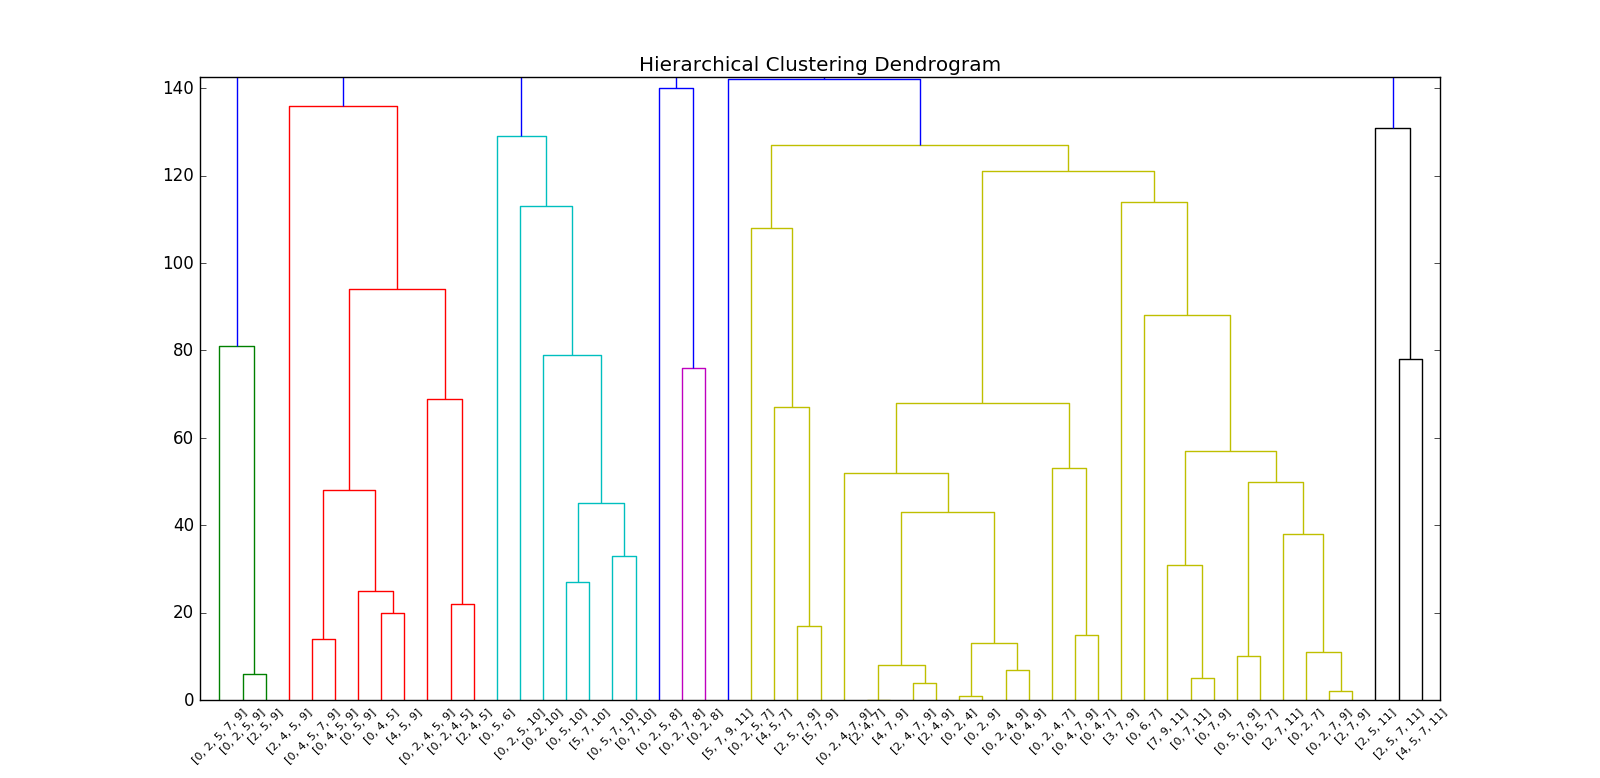
\includegraphics[width=6in]{Dend_ii_IV_I_vi_V.png}
	\caption{Close-up of Figure~\ref{Dend_complete}.  Color-coded clusters here capture categories corresponding to traditional scale degree set descriptions of $ii$, $IV$, $I$, $vi$, and $V$.  Note that the clustering algorithm knows only the behavior of the chords -- not their pitch class content.}
	\label{Dend_sub1}
\end{figure}
%iv appears in both of the below.  Is this because iv behaves differently in major vs. minor key contexts?
\begin{figure}
	\centering
	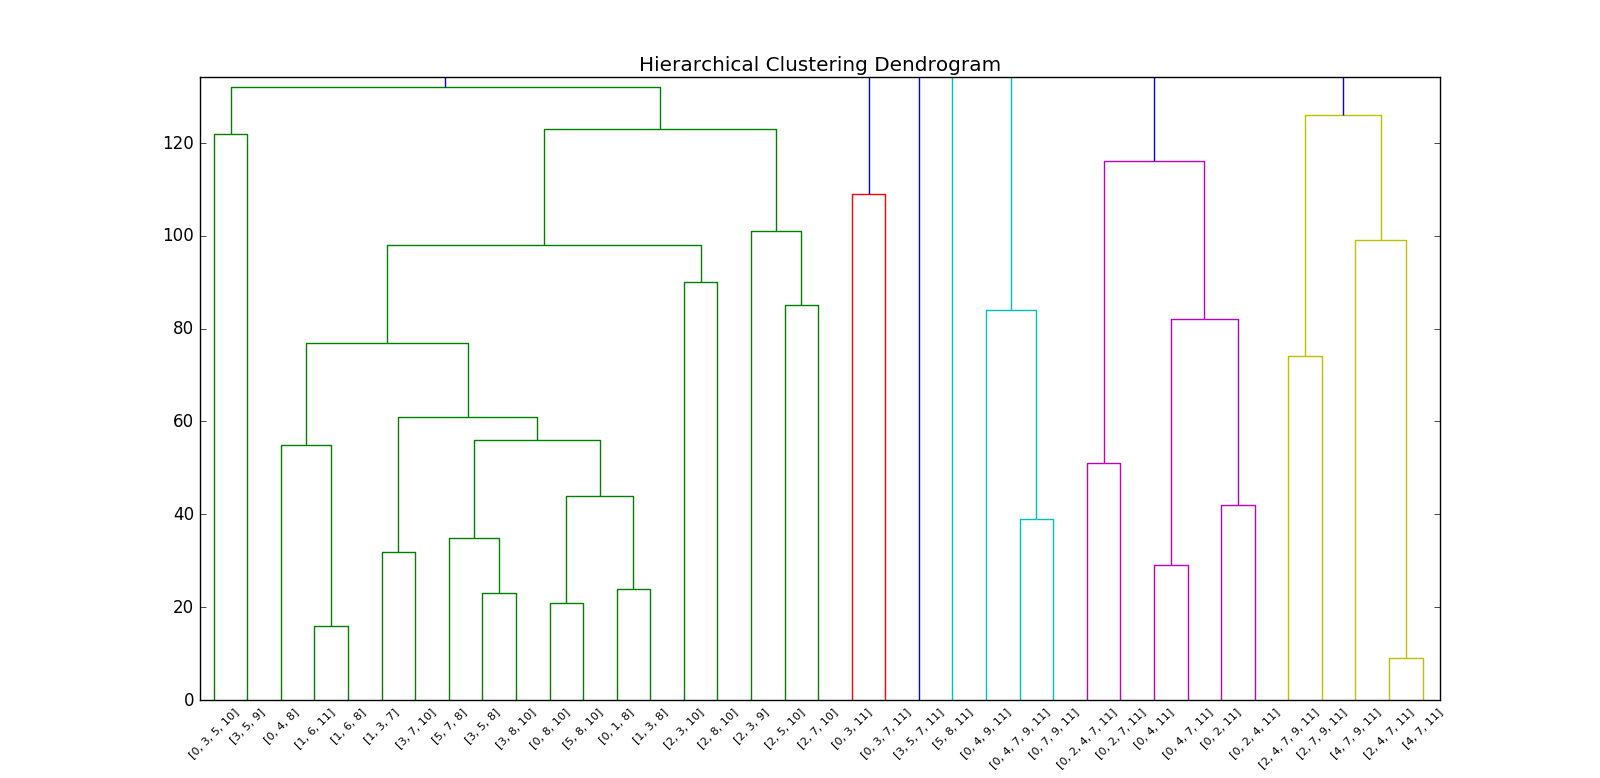
\includegraphics[width=6in]{Dend_iv_I7_iii.png}
	\caption{Close-up of Figure~\ref{Dend_complete}.  Color-coded clusters here capture categories corresponding to traditional scale degree set descriptions of $iv$, $I^7$, and $iii$.  Note that the clustering algorithm knows only the behavior of the chords -- not their pitch class content.}
	\label{Dend_sub2}
\end{figure}

Figure~\ref{Dend_sub2} contains a similar range of functional clusters.  At right are several clusters containing the leading tone ($[11]$ or $\hat{7}$).  The yellow cluster contains varieties of $iii^7$, like $[2,4,7,11]$ and $[4,7,11]$, as well as pitch class sets we might describe as root-ambiguous, or both $V$-like and $iii$-like.  The agglomerative clustering here sidesteps whether $[2,4,7,9,11]$ should be described as a $V$ triad with added sixth and ninth (less likely, due to the missing chordal seventh, but logically permissible) or as a $iii^{11}$; of importance to the clustering is that the scale-degree set behaves in a way very similar to the other chords in the cluster, several of which resemble traditional $iii$ chords.  The purple and cyan clusters on the right hand side of Figure~\ref{Dend_sub2} also contain tonic-type chords.  The majority of the purple cluster consists of $I^7$ voicings, while the chords of the cyan cluster typically feature the addition of $\hat{6}$ (i.e., the purple cluster contains $[0,4,7,11]$, while the cyan cluster contains $[0,4,7,9,11]$).  Both the purple and cyan clusters separate the voice-leading behavior of major tonics containing leading tones from Figure~\ref{Dend_sub1}'s cluster of leading-tone-free tonics, and all three of the of the clusters at right on Figure~\ref{Dend_sub2} are similar enough to merge at the next branching point up the hierarchical tree.

Figure~\ref{Dend_sub3} shows a variety clusters suggestive of minor keys and ``flat-side" harmony.  In the cyan cluster near the middle, $[0,3,7]$, $[0,3,10]$, and $[0,3,7,10]$ appear adjacent to one another -- the three most common scale-degree expressions of the minor tonic chord.  The remainder of the cyan cluster indicates that the addition of scale degree $\hat{4}$ (in chromatic semitonal notation, $[5]$) to minor tonic chords leaves their progression statistics relatively unchanged.  While $[0,3,7]$, $[0,3,10]$, and $[0,3,7,10]$ fall in the left cyan ``subcluster," $[0,3,5,7]$, $[3,5,10]$, and $[0,3,5,7,10]$ all fall in the right.  This clustering appears to support the ``extended harmony" dictum that perfect 11ths may be added to minor chords without significantly altering their functional properties.  The purple cluster to the right contains many instances of minor tonic scale degrees $\hat{1}$, $\flat\hat{3}$, $\hat{5}$, and $\flat\hat{7}$ ($[0,3,7,$ and $10]$), but with the frequent addition of $\flat\hat{6}$ ($[8]$).  This includes chords that might carry roman numeral label $\flat VI$, like $[0,7,8]$ and $[0,3,7,8]$, as well as more ambiguous collections of minor key scale degrees, like $[7,8,10]$ and $[2,7,8]$.  This cluster's composition does not necessarily indicate that the chords appear exclusively in minor keys; rather, it demonstrates that they progress the same way over time, whether as modal mixture in major key contexts, flat-side modulatory passages, or as diatonic minor harmonies.

%Weird clusters
Aside from recognizably predominant, dominant, and tonic clusters in major and minor modes, the agglomerative clustering of Figure~\ref{Dend_complete} provides both a framework for categorizing systematically-used chords of lower probability and an indication of where the limits of cluster interpretation might lie.  The cyan cluster on the left hand side of Figure~\ref{Dend_sub1} contains a collection of chords bearing family resemblance, where no single scale degree or root occurs across all members of the cluster.  Most of the chords contain scale degree $\flat\hat{7}$, whether as part of a $v$ (like $[5,7,10]$) or a scale-degree set potentially identifiable as $\flat VII$ (like $[0,2,5,10]$), and each chord contains at least two scale degrees in common with its nearest neighbors.

%Green cluster of Figure~\ref{Dend_sub2}.  Has a lot of [8] in it?  Some bVII and v?  Possible junk drawer?
The green cluster at the left hand side of Figure~\ref{Dend_sub2} elevates the ambiguity of traditional interpretation to levels which cast doubt on the utility of the cluster.  Here, scale degree sets corresponding to $v$ ($[2,7,10]$) and $\flat VII$ ($[2,5,10]$) share a large cluster with root-third-seventh voicings $[3,5,8]$ and $[3,5,9]$.  The latter might be interpreted as a $V^7 / \flat VII$, and several other flat-side chords relative to that key area also appear (like $[3,7,10]$), but the cluster otherwise bears some resemblance to a ``junk drawer," a cluster into which the algorithm dumps noisy chords with complex behavior.

None of the chords in this green cluster are among the top 100 most unigram-probable chords except $[2,7,10]$, $[2,5,10]$, $[3,5,8]$, and $[3,7,10]$, a fact which reflects the increasing difficulty of clustering lower-probability chords in an intuitively (or syntactically) meaningful way.  When the agglomerative hierarchical clustering algorithm is given a large number of low-probability chords to tag with cluster labels, the perceived syntactic consistency of the clusters begins to break down.  Under such conditions, investigations into the potential behavior of low-probability chords benefit from \emph{supervised} machine learning classifier methods, where the initial clustering of high-probability chords is taken as a given, and new chords are categorized with respect to the initial framework. 

\begin{figure}
	\centering
	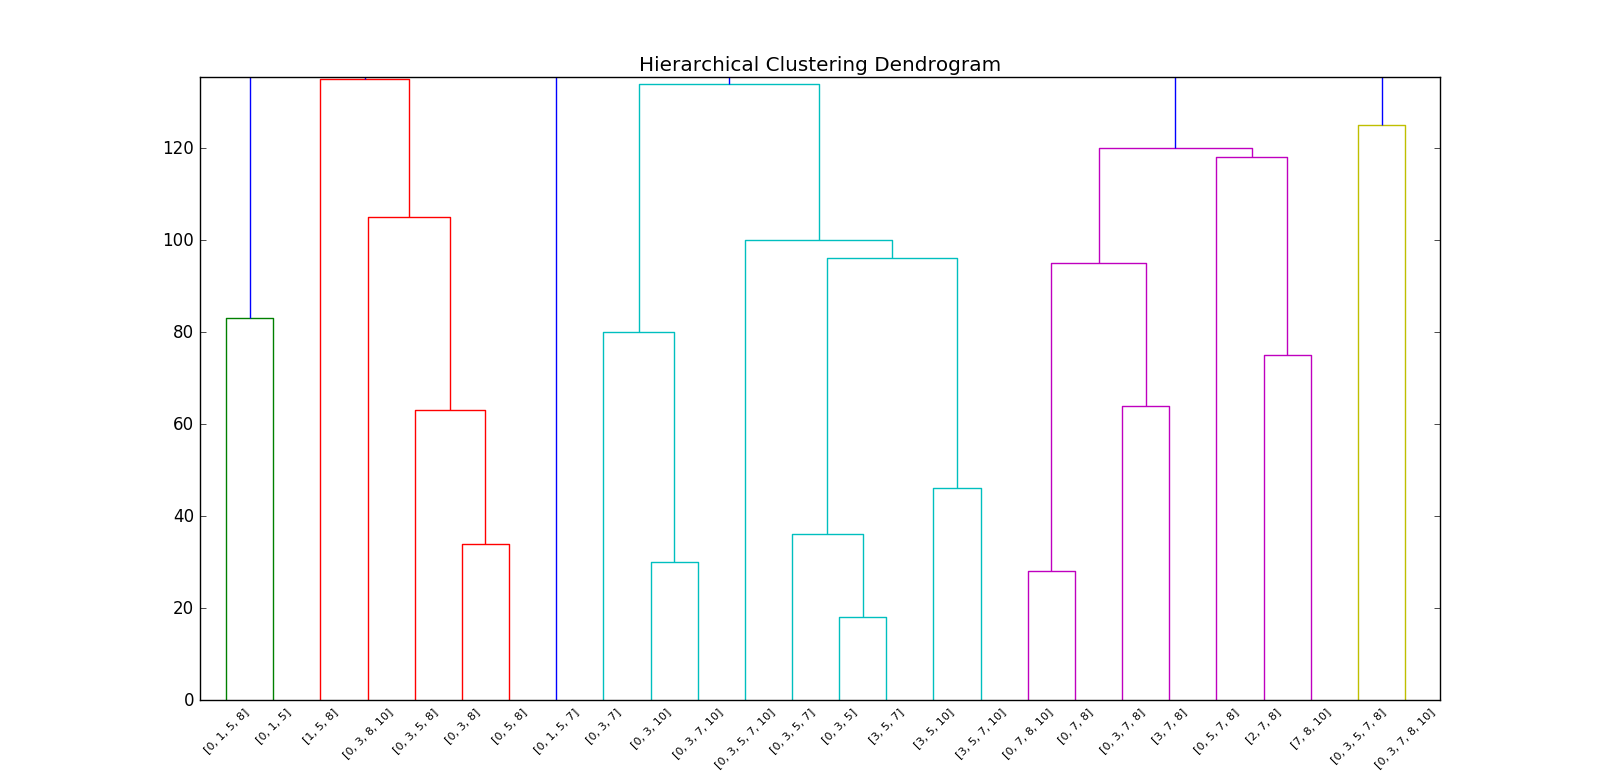
\includegraphics[width=6in]{Dend_iv_bVI_i.png}
	\caption{Close-up of Figure~\ref{Dend_complete}.  Color-coded clusters here capture categories corresponding to traditional scale degree set descriptions of $iv$, $\flat VI$, and $i$.  Note that the clustering algorithm knows only the behavior of the chords -- not their pitch class content.}
	\label{Dend_sub3}
\end{figure}

%TODO: add table of full dendrogram membership, for readability (and numerical cross-ref)

\section{From categories to classifications}
%Lay out the general problem: want to get categories without noise -- especially so we can see useful behavior -- but then also use those categories for classifying noisier states
%Note that various types of machine learning algorithm can place lower-P chords into the flat agglomerative clustering classes; don't come down on one firm algorithm.
%MAYBE: Then note that training on high-P chords allows us to see some of what categories "do" (cat-to-cat transitions?)
Given a set of meaningful category assignments for high-probability chords, as introduced in the previous section, lower-probability chords may be classified into these categories by machine learning algorithms trained on the set of high-probability category assignments.  Supervised machine learning algorithms take a predictive stance with respect to ``new" observations, using patterns gleaned from known classifications to guess what tag should be assigned to a previously unseen observation.  Different specific algorithms accomplish the task in different ways, but each ``learns" from a training set -- high-probability chords and their cluster assignments, in this case -- and then attempts to extrapolate that learning to make predictions about sensible class assignments for elements of a testing set -- here, lower-probability chords not captured by the initial clustering.

Two important kinds of optimization confront any analyst choosing from the wide variety of supervised classifiers.  First, the utility of a given classifier is typically assessed by examining how well it performs on a subset of the data for which the desired category assignments are known.\footnote{Give a source for cross-validation?}  In the case of YJaMP's syntactic clustering, this cross-validation scheme involves separating the flat clustering itself, in which all of the 200 most probable chords receive cluster assignments, into distinct training and testing sets.  If a machine learning algorithm is trained on a random selection of 80\% of the top 200 chords, comparing their temporal probability matrices to their cluster assignments in order to generate a predictive model mapping the former to the latter, it can then be tested on the remaining 20\%, chords which the model has never seen.  Since the flat clustering nevertheless provides category assignments for these chords -- assignments the machine learning model did not see or use in its predictions -- the accuracy of the model's predictions for the ``held out" 20\% can be calculated by comparing the predicted cluster assignments to the real, pre-existing assignments made by the flat clustering algorithm.  Moreover, this validation process can be automated and repeated with new choices of 80/20 splits, decreasing the importance of any particular random selection within the training set.  The average accuracy across many such splits provides a measure of how well a particular class of supervised machine learning classifier performs -- and thus how well it should be trusted to predict cluster assignments for the unknown chords outside the top 200 most probable.

%Do I need to define accuracy/precision/recall?

Such cross-validation applies to any supervised classifier, providing a metric with which to choose between different algorithms.  Each algorithm, however, can be fine-tuned in a number of ways.  Most depend on several model parameters set \emph{a priori}, the effect of which on the model's predictive power may itself be difficult to predict.  This second kind of optimization, in which the analyst attempts to choose the best parameters for a given model, can make use of cross-validation as a tool for assessment -- but the cross-validation must be performed for each plausible combination of model input parameters, or at least some meaningful subset of that parameter space.

Fortunately, scikit-learn provides ready-made Python methods for both repeated, automated cross-validation and optimization over model parameters.  With the flat cluster assignments as tags for each of the 200 most probable chords in YJaMP, I employ two main scikit-learn methods: \emph{train\_test\_split} randomly divides the clustering into an $80\%$ development/training set and a $20\%$ testing set, and \emph{GridSearchCV} checks a wide variety of model parameters via cross-validation on the training set.  Given a ``grid" consisting of many combinations of model parameters, GridSearchCV uses every possible combination of those input parameters to build a model based on the development set.  It employs a multi-fold cross-validation scheme, where the development set is divided into four different parts, and each part is sequentially ``held out" as an internal testing set.\footnote{Formally speaking, I employ \emph{stratified} k-fold cross-validation, since the cluster sizes in the training data are unbalanced; this attempts to preserve the rough proportions of each cluster in each fold.  And since some very small clusters cannot be divided into separate folds, the algorithm throws out clusters with fewer than three observations in them.}  Based on each parametric model's performance in the cross-validation, GridSearchCV chooses the set of parameters most likely to yield a high-accuracy model on the final testing set.  Put another way, the model selection process follows a series of steps:

\begin{enumerate}
	\item Divide the overall flat clustering into a development set ($80\%$) and a testing set ($20\%$).
	\item For a given supervised classifier type, choose a grid of parameters over which to optimize.
	\item For each combination of parameters, divide the development set into four equal and randomly selected ``folds" for cross-validation.
	\item Treat each of these folds as a testing set, sequentially; when fold 1 is the testing set, train the model on folds 2-4; when fold 2 is the testing set, train the model on folds 1, 3 and 4; etc.
	\item Calculate the average accuracy score across all folds for a given combination of model parameters.  Select the parameters which yield the best score.
	\item With model and parameters in hand, train the selected classifier on the full development set and test it on the originally held-out testing set.
\end{enumerate}

%set up and explain k-nn example, which is definitely the simplest appropriate classifier
The ``k-Nearest Neighbors" algorithm (kNN) constitutes the simplest machine learning technique compatible with the above training and testing pipeline.  In some ways, kNN stands as a limiting case for machine learning algorithms, in that it requires the construction of no explicit model at all -- training the algorithm only requires storing the tagged training set and defining a way to determine what members of that set are closest to a new observation in need of a label.  When a kNN algorithm encounters an observation in the test set which needs a category tag, all it does is look through the training set to find the closest tagged observations.  It then assumes that whatever tag the clusterer applied to its nearest neighbors should also apply to the (previously untagged) test case.

Building a development set from a random selection of $80\%$ of the tagged destination chord matrices, I subject kNN to a parameter grid search with a small range of possible variables over which to optimize (step (2) above).  First, the algorithm can consider any number $k$ of the nearest neighbors to a given test observation when making its tag prediction; I preselect values of $k$ ranging from 1 (the closest neighbor only) to 10.  While selecting those neighbors, I allow the algorithm to employ either a Manhattan or Euclidean distance (both cases of general Minkowski distances with $p=1$ or $p=2$, respectively).  And in cases where the algorithm considers more than one neighbor ($k>1$), it allows the neighbors to ``vote" for a winning tag using either of two weighting schemes: each of the $k$ neighbors suggests its tag with equal weighting, or each suggests its tag with a weighting inversely proportional to its distance from the test observation.  If the algorithm considers the five nearest neighbors to a test observation, for example, the former case would ask each neighbor to vote once with its classification tag, and the resulting tally would determine the winning prediction.  With distance-based weighting, however, the closest single neighbor's vote carries more weight than each of the other four, and the tag with the largest total \emph{weighted} tally determines the prediction.

With these relatively crude parameters, gridSearchCV builds kNN models on the development set.  As steps (3) and (4) above indicate, each model stores three-quarters of the development set in order to ``train" the model.  Each of the remaining chords in the development set is then compared to the training set with the given choice of model parameters.  The predictions made based on the training portion of the development set are compared to the actual tags for the remaining observations, and an accuracy measure is tallied.  The kNN model parameters which tend to yield the highest accuracy scores are then reported (step (5))-- and a model with those parameters may then be trained on the full development set for use on the originally held-out $20\%$ test set (step (6)).

%gridSearch kNN selections: p = 1, neighbors = 1 or 3, weights = uniform or distance
Given the simplicity of the original clustering algorithm, it comes as no surprise that the grid search suggests simple optimal parameters for the kNN model: with a wide variety of initial random splits for the data set, gridSearchCV only suggests two possibly optimal combinations.  For most trials, the most accurate model chooses to consider only the closest single neighbor ($k=1$) under the Manhattan distance metric.  In a smaller number of trials, the model selects the three closest neighbors ($k=3$) and weights their votes in inverse proportion to their Manhattan distance from the test observation.  The cross-validation accuracy scores for these models within the development set tend to fall in the range $0.55 \pm 0.1$; this indicates that if a model trained on the development set were used to predict values for the test set, we might expect a similar level of accuracy.

Running this procedure 100 times, where a model is trained and optimized on the development set and then used to predict tags for the test set, produces a range of accuracy scores plotted in Figure~\ref{kNN}.  As the cross-validation scores predicted, the accuracy on the test set centers around $57\%$, falling off steeply within about $10\%$ on either side.  This means that across the (randomly selected) test set, the model typically guesses the correct category assignment between one half and two thirds of the time.

%Perform this optimization many times and give a histogram of the accuracy on the testing set.  This makes clear that I'm not cherry-picking accuracy.
\begin{figure}
	\centering
	\caption{A histogram capturing the accuracy of 100 grid search optimized k-Nearest Neighbors classifiers applied to different 80/20 development/testing set splits.}
	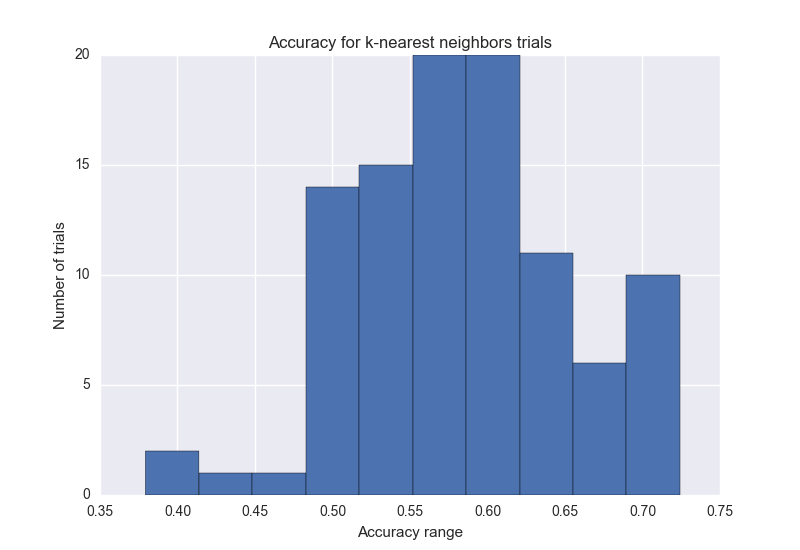
\includegraphics[width=4.75in]{kNN_acc.png}
	\label{kNN}
\end{figure}

The types of predictions the model makes reveal where the largest sources of error are.  A classification report for a typical set of model predictions (accuracy $59\%$) is given in Table~\ref{class_report}.  The first column of the table references category numbers assigned by the flat clustering algorithm alongside a hand-chosen, roughly representative scale-degree set of that category.\footnote{Again, neither the clusterer nor the classifier store or employ any notion of a paradigmatic representative for chord categories; this is purely a human heuristic.  A clustering algorithm like k-medoids, on the other hand, \emph{would} choose such a representative for each cluster.  Exploratory k-medoids clustering code for YJaMP can be found in \href{https://github.com/andrewdjones/YJaMP_Analysis/blob/master/yjampClus.py}{yjampClus.py}.}  The cluster numbers themselves are meaningless, though their ordering and adjacency reflect higher-level cluster similarities in the hierarchical model.

For each category, the classification report provides precision and recall scores alongside the category's ``support," the number of members of the category which appeared in this particular test set.  Precision and recall refer to complimentary accuracy metrics.  For each row on Table~\ref{class_report}, the model's recall refers to what percentage of the test observations from the category the model classified correctly; a score of $1.0$ indicates that each of the members from the category appearing in the test received the appropriate cluster label.  Precision tracks the model's ``false-positives."  Since cluster 12, a large tonic cluster, contains many samples (6 appear in the test set), a na\"{i}ve first-order (non-kNN) model might attempt to label \emph{all} observations with the tag ``12."  This would guarantee perfect recall for category 12, but it would result in a large number of other observations erroneously receiving the same tag.  The precision score tracks what percentage of the model's guesses for a given category tag turned out to be correct.  A precision of $1.0$ indicates that every time the model guessed a particular tag, it was correct, while a precision of $0.5$ indicates that half of the model's assignments of a particular category tag were incorrect (even if the correct applications capture $100\%$ of the actual members of the intended category).

The model's best performance seems to correlate with tonic-type chords, like those in categories 12, 19, 20, and 53, while the model guessed no correct tags at all for several categories (9, 10, 18, 36, 37, 51).  The comparatively low precision scores for categories 12 and 15 indicate that many of the mis-identified observations received tags from these categories.  The model's many guesses and high recall scores for categories 12 and 15 reflect that these are the largest categories in the training set (and the corpus in general); the flat clusterer grouped 27 of the top 200 most probable scale-degree sets into category 12, and 19 into category 15, so the kNN model is more likely to find a nearest neighbor here than in another category -- especially a category with few members.

\begin{table}%[h]
  \caption{Classification report for a grid search-optimized k-Nearest Neighbors test predicting the category tags for 29 previously-unseen chords.}
  \centering
\begin{tabular}{l |l |l |l }
\hline\hline
cluster & precision	&  recall &  support \\ [0.5ex]
\hline
	 9 $[0,4,5,9]$	    &    0.00  &    0.00   &       2\\
	 10 $[5,7,10]$  	&    0.00  &    0.00   &       1\\
	 12 $[0,4,7]$		&    0.56  &    0.83   &       6\\
	 15 $[3,5,8]$ 		&    0.43  &    0.75   &       4\\
	 18 $[0,4,7,9,11]$  &    0.00  &    0.00   &       1\\
	 19 $[0,4,11]$		&    1.00  &    1.00   &       1\\
	 20 $[4,7,11]$		&    1.00  &    1.00   &       1\\
	 35 $[2,6,7,11]$	&    1.00  &    1.00   &       1\\
	 36 $[2,4,8]$		&    0.00  &    0.00   &       1\\
	 37 $[0,4,10]$	    &    0.00  &    0.00   &       2\\
	 38 $[0,2,6]$	    &    0.50  &    1.00   &       1\\
	 42 $[2,6,9]$	    &    0.50  &    0.50   &       2\\
	 48 $[0,2,5]$	    &    0.50  &    0.50   &       2\\
	 51 $[0,3,5,8]$	    &    0.00  &    0.00   &       1\\
	 53 $[0,3,7,10]$    &    1.00  &    1.00   &       2\\
	 54 $[0,3,7,8]$	    &    1.00  &    1.00   &       1\\
\hline
avg / total  &  0.47   &  0.59   &       29\\[1ex]
\hline
\end{tabular}
\label{class_report}
\end{table}

%reminder that this is not a human
These classifications are certainly not as accurate as those made by a suitably-trained human analyst, but they are produced by an entirely different and much more na\"{i}ve process.  A trained kNN model provides proof of principle that lower-probability chords -- for which the flat clustering algorithm provides no tag at all -- can still be assigned a classification within the scheme of the clustering.  The complex temporal behavior of the most probable chords in a corpus can be used to produce a bottom-up agglomerative clustering, and then a machine learning model can use that clustering to make (imperfect, but much better than random) decisions about rarer chords.

%give predictions for a couple of low-P chords
Many of the scale-degree sets with probability rank 200-300 in the corpus suggest no clear interpretation to a human analyst, so it can be difficult to assess whether or not the tags assigned to them by the basic kNN model are useful.  Some predictions appear accurate and sensitive: $[0,2,4,5,7]$ is assigned to category 12, the ``tonic-without-major-seventh" category, while $[0,2,7,9,11]$ is assigned to category 19, where the $I^7$ scale-degree sets appear -- and this based only on progressions statistics, not pitch-class similarity.  But many scale-degree sets receive tags for categories 12 and 15, and the low precision displayed by kNN models cross-validated on the development set indicates that many of these applications are spurious.  The minimally-informed learner, our distance-based k-Nearest Neighbors algorithm, lacks a sophisticated algorithmic ear.

%drawbacks
Several roadblocks stand in the way of the model's performance.  Nearest-neighbor models make poor generalizers, since they are explicitly and only sensitive to the structure of the data on its most local scale.  Beyond the choice of $k$ neighbors and a weighted distance, no other points or features from the training set guide the choice of tag assignment.  Moreover, the representation and sensitivity of the input data is poorly suited to the choice of metric.  The element-wise Manhattan distance between two destination chord matrices -- used by both the flat clusterer and the kNN classifier -- essentially flattens out each matrix into a long, 600-element vector.  The ``feature space" in which these vectors live is enormous, while the number of data points with which the models can be trained is comparatively tiny, suffering from the ``curse of dimensionality."\footnote{In general, training a 600-dimensional model on fewer than 200 observations is a terrible idea.  It only works even as well as it does here due to (1) the shared metric between clusterer and classifier and (2) the variance concentration provided by PCA.}  If the model knew in advance, for example, that the PCA1-scores of each (or many) destination chord(s) in the matrix might scale and behave similarly, or that the PCA-2 scores might do the same, more efficient heuristics might be encodable which would reduce the overall dimensionality of the input data and structure the models which might be built from it.

%metric learning
More advanced machine learning techniques may mitigate both of these problems, up to a point.  Metric-learning approaches can suggest more sensitive (i.e., non-Minkowskian) distance metrics (and pseudo-metrics) learned from the tagged training set.\footnote{For an overview and relevant Python tools, see the documentation for the package \href{https://github.com/all-umass/metric-learn}{metric-learn}.}  Such a metric might treat different dimensions of the data differently in order to place similarly-tagged observations as close together as possible, improving the accuracy of a kNN-type model. 

%tensor structure and neural networks
To take advantage of any structure embedded in the two-dimensional destination chord matrix representation, a subtler classifier could draw on machine learning models developed for image processing applications, many of which treat each image as a \emph{tensor}, rather than as a flattened vector.\footnote{While vectors constitute first-order tensors, most out-of-the-box machine learning algorithms do not readily generalize to higher-order tensor inputs.}  While vector representations associate each origin chord with a single vector in a very high-dimensional space, tensor representations preserve the multi-dimensional structure of the input data (matrices, in this case, which are second-order tensors).  Research on tensor-based classification problems like image recognition, where each pixel in an image might carry several features like position and color, indicates that preserving tensor structure permits the use of learning algorithms trainable with a smaller data set.\footnote{This mostly boils down to the multilinear algebraic efficiency of using several linear transformation matrices to reduce the dimensionality of a large tensor, compared to one much larger linear transformation matrix necessary for high-dimensional vector reduction.  For a helpful overview of the math behind (especially linear-kernel) supervised tensor learning, see Tao et al 2006; for further (especially nonlinear-kernel) image-recognition application examples, see He et al 2014.  These approaches have been applied to musical genre classification problems (Panagakis, Kotropoulos, and Arce 2009), but not to syntactic progression data.}  In particular, support vector machine-type models, which attempt to calculate (hyper)planes of greatest separation between data subsets for classification, generally require a much larger training set than a corresponding support tensor machine for problems amenable to tensor representation.\footnote{See He et al (2014).}

%explain clusterer-classifier alignment in Kockelmanian terms
But a classifier with increased sensitivity would be limited by both the results of the initial clustering algorithm and the data representation scheme.  Moreover, the degree to which the classifier's performance might be deemed ``better" would depend on human analytical interactions with the algorithmic agents.  In the Kockelmanian terms introduced in chapter 2, any data pipeline entangles several distinct agents, some human and some non-human, in the production of objects, signs, and interpretants.  For any supervised classifier based on a prior clustering scheme of any arbitrary sensitivity, the training of the model involves communication between the two algorithmic agents in a specifically semiotic sense -- and the selection processes employed by both agents depend on the scale-degree set parsing performed by other and earlier algorithmic agents.  

\section{Algorithmic semiotics and data pipelines}
Some of the modes of mediating interrelationality within this network of activity can be read onto the Kockelman graph reprinted as Figure~\ref{kockelman_3dia}.

\begin{figure}%[h]
	\centering
	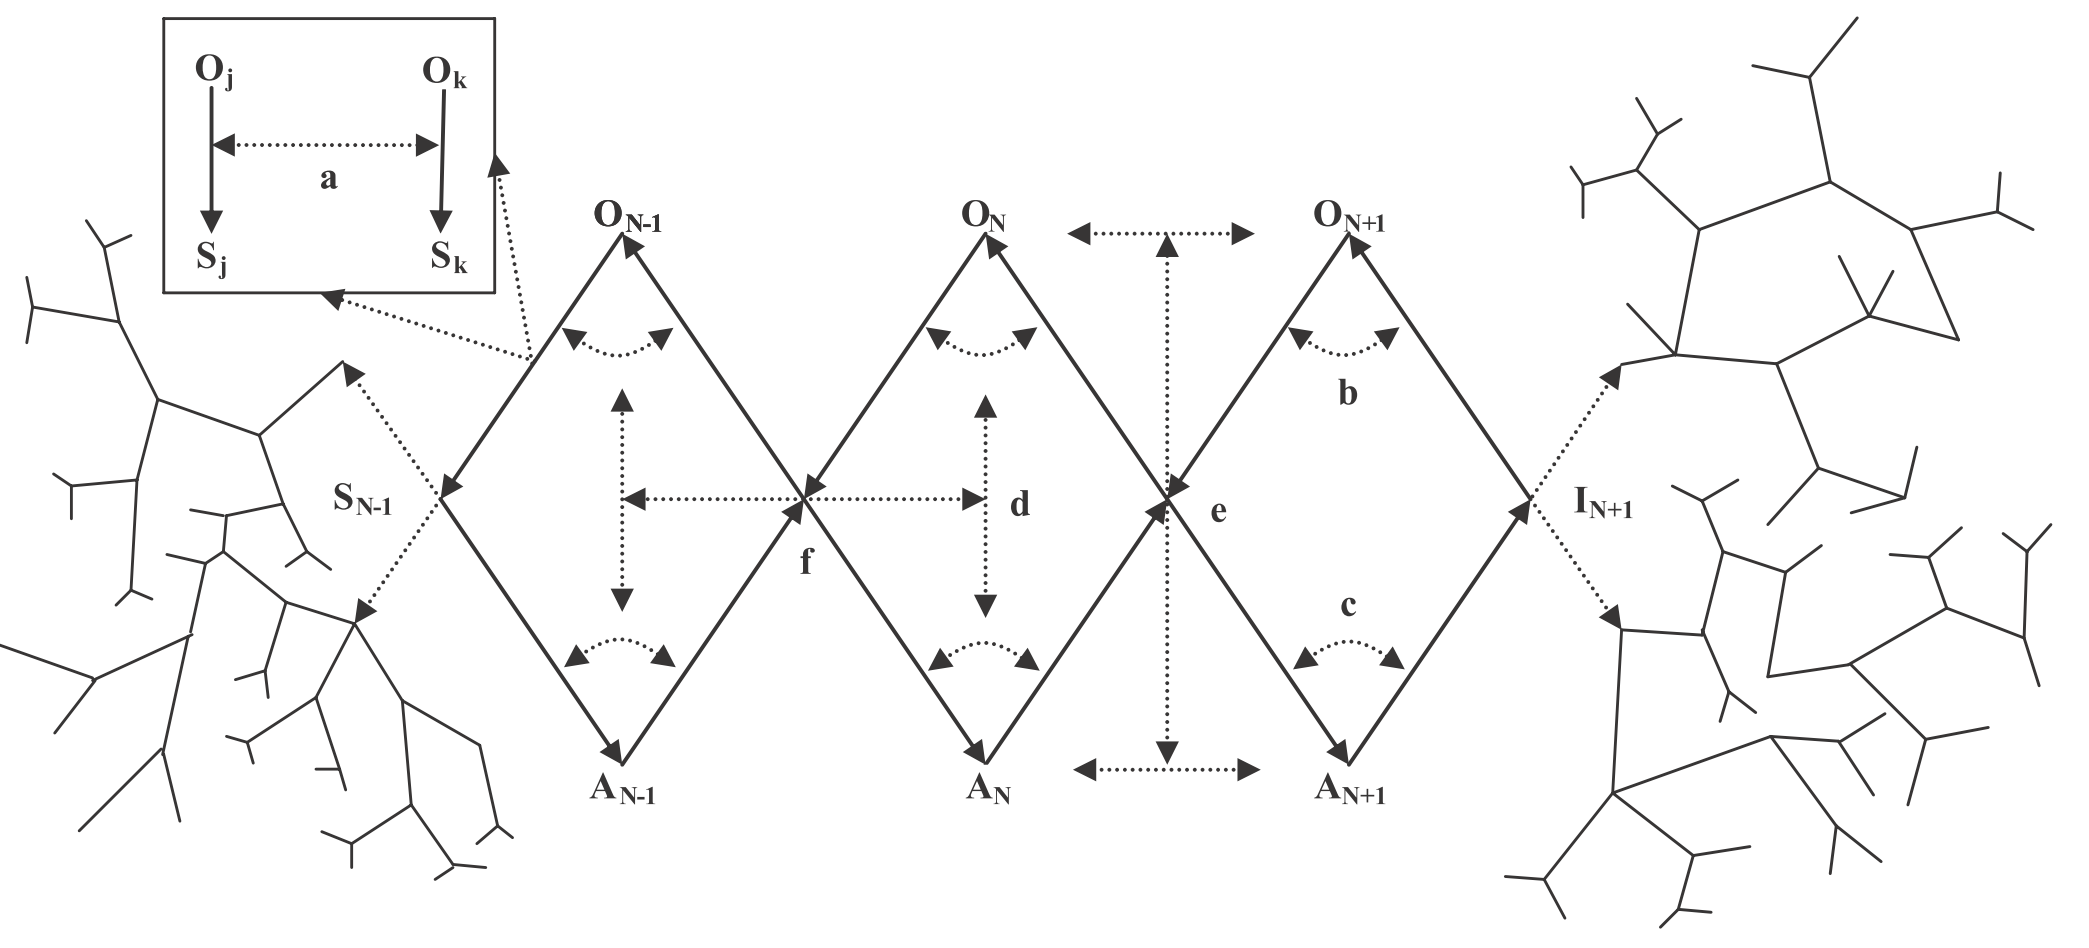
\includegraphics[width=5.5in]{kockelman_3dia.png}
	\caption{Figure 2.9 from Kockelman 2012, a graph of ``relations between relations revisited."  In a complex, rhizomatic network of agents, we might envision $A_{N-1}$, $A_N$, and $A_{N+1}$ as a scale-degree set tallier, an unsupervised clustering algorithm, and a supervised classifier, respectively, though the chain of agents involved in the analytical ecosystem necessarily extends further back (MIDI boxes, pianos, pianists, printers, composers), forward (jazz syntax theorists, pedagogues, harmony students, pianists), upward (music information retrieval, meta-theory, acoustics), and downward (code porting, algorithmic optimization, psychological experimentation, pedagogy research).}
	\label{kockelman_3dia}
\end{figure}

%parser, clusterer, classifier do different things, communicate in certain ways, 
%A_{N-1} = scale-degree set tallier	& O_{N-1} = scale-degree set & I_{N-1} = destination chord TPDs
%A_{N} = clusterer & O_{N} = ``collection of $m_1$-similar high-probability scale-degree sets"  & I_{N} = cluster
%A_{N+1} = classifier & S_{N+1} = tagged TPDs, untagged TPD & O_{N+1} = ``collection of $m_2$-similar clusters" & I_{N+1} = category assignment
%A_{N+2} = human analyst & S_{N+2} = traditional chord functions, cluster assignments & O_{N+2} = ``clusters with function-mappable scale-degree set members" & I_{N+2} = category syntactic functions
Each communicative translation across the network imbricates an agent and a set of signed indices in the production of an interpretant.  After some undefined (and likely very large) number of agents produce the corpus -- composers, record labels, fake-book printers, pianists, MIDI boxes -- Figure~\ref{kockelman_3dia} might be used to depict the scale-degree set tallying agent as $A_{N-1}$.  Note that this agent itself could be decomposed into several separate routines in communication through their own indices and interpretants, like the perplexity-based time-window calculator and the key-finding transposer (say, $A_{N-1,1}$ and $A_{N-1,2}$).  The scale-degree tallying algorithm interprets MIDI files, with indices of pitch and time ($S_{N-1}$), to produce statistics for how often scale-degree sets follow one another at particular temporal delays: temporal probability distributions $I_{N-1}$ for each origin chord.  These interpretants make sense from the perspective of the tallying agent in the presence of particular pitch and time indices given the properties of scale-degree sets as chord objects $O_{N-1}$.  The $O_{N-1}$ are identified by each particular signed presence of several scale degrees relative to the pitch-profile determined local key, and they have other, similar objects which follow them in time.  Note also that, for $A_{N-1}$, the various origin chords are bundles of pitch and time features constructed with no other features: they are not like or unlike one another; they are not substitutable; they are not consonant or dissonant; they are not \emph{Stufen} or voice-leading neighbors.

The temporal probability matrices produced by $A_{N-1}$ stand as indices for the clustering algorithm $A_{N}$, which otherwise knows nothing about MIDI files, key profiles, or individual tunes.  The clustering algorithm produces clusters $I_{N}$ of scale-degree sets it deems similar to one another.  The clusters make sense given the temporal probability matrices if and only if the clusterer assumes (or generates) the existence of objects $O_N$ that we might call ``collections of metric $m_1$-similar high-probability scale-degree sets."  No interpretants indicating similarity between different origin chord temporal probability matrices are possible without the choice of some metric for comparison; the way in which the metric properties of the interpretant clusters relate to the matrices which represent their elements precisely and necessarily balances the sense-making of the clusters given the matrices from the perspective of the algorithm.  This relation-between-relations corresponds to arrow $(d)$ on the figure.  The properties of $O_N$ and the knowledge of $A_N$ are co-determinate across this relation-between-relations.  For this semiotic process, neither those properties nor that knowledge exist independently.

Since the tallier and clusterer are both Python algorithms treating particular kinds of computational processes (like list-building, arithmetic, memory management, string matching), the sign-object-interpretant to sensation-agent-instigation relations $(d)$ underpinning the activities of each are subject to certain similarities.  ``The subset of relations marked $(f)$," as Kockelman explains, ``... may be understood as relations between relations of type $(d)$ as constituted by an ensemble of interconnected envorganisms-- be they neurons or logic-gates, speech acts or mental states, instruments or actions, intentional individuals or sieving gradients."\footnote{Kockelman 2012, p.\ 38.}  Kockelman uses the term ``envorganism," an environment-organism hybrid, to call into question any straight-forward \emph{a priori} division between individuals and their contextual environments.  A clustering algorithm produces cluster objects as much as it depends on them, and it does so in a way similar to the interactions between other algorithms and their respective ontologies.  This similarity in semiotic processes constitutes code-like channels recognizable as the shared infrastructure of Python scripts in general.\footnote{Kockelman in fact casts ``channels" as generalizations of Saussure's languages-as-codes in general, where Saussure's relations between object-sign pairs (arrow $(a)$ on Figure~\ref{kockelman_3dia}) are replaced by the relations between semiotically-similar envorganisms (themselves constituted by relations between relations) given by arrow $(f)$.}

The clusters produced by $A_N$ themselves serve as signs interpretable by the classifier $A_{N+1}$.  In the particular k-Nearest Neighbors case, the classifying agent $A_{N+1}$ took tagged temporal probability matrices as signs standing for objects an unseen/untagged scale-degree set might be `like."  Given the existence of a collection of clusters with degrees of similarity or appropriateness $m_2$ to the untagged observation chord, the classifier produces a new tag as an interpretant.  The sense-making of the cluster tag assignment $I_{N+1}$ depends on another metric, $m_2$, which may or may not align with the sense-making metric $m_1$ employed by (and constituting) the clusterer $A_{N}$.  In the kNN case, I employed a metric $m_2$ precisely the same as the clusterer's metric $m_1$ -- both Manhattan distances on flattened vectors -- and this choice produced particular relations between the clusterer/classifier ($A_N$ and $A_{N+1}$) and their co-constructed objects ($O_N$ and $O_{N+1}$).  In particular, as Kockelman's arrow $(e)$ depicts, the relation between the two agents is ``mediated by a relation between things."\footnote{Kockelman 2012, p.\ 38.}  If the objects co-constructed by the two agents both rely on Manhattan metrics, then the classifying agent relates to the clustering agent quite closely, assigning tags to and in light of the same kind of cluster objects that gave rise to the interpretants $I_N$.  But if $m_2 \neq m_1$, the relation between the classifier and clusterer becomes less clear, more strongly mediated by the relation between the two types of cluster category invoked and produced.  A classifying algorithm more sensitive than or differently constituted from the clusterer operates with different ontological conditions, and any attempt to train and evaluate the classifier will need to compare potential incommensurables.  To ask an intensely circular question: if a highly-sensitive classifier is trained on the results of a poor clusterer and produces a predicted tag which disagrees with that given by the clusterer, which one is to be trusted?

At each step of the data analytical pipeline diagrammed in Figure~\ref{kockelman_3dia}, slightly different objects and agents relate to signed indices and instigated interpretants, and the relations between any two agents are mediated by the relations between their respective co-constructed objects.  Which of these objects are chords with syntactic function?  Which carry properties corresponding to those specified and employed by human-analytical agents?  In an important sense, any human interpretation of the results of such a pipeline \emph{is itself part of the pipeline}.  A tonal jazz syntax analyst $A_{N+2}$ treats the interpretants $I_{N+1}$ and $I_N$ produced by algorithms $A_{N+1}$ and $A_{N}$ (and dependent on $A_{N-1}$ and $A_{N-2}$ and...) as signs indexing particular objects $O_{N+2}$, which might be ``clusters with function-mappable scale-degree set members."  By assuming and generating such objects, the human analyst can then assess the algorithmic interpretants in order to assign an intuitive notion of ``syntactic function" to the clusters or tagged scale-degree sets.  The algorithms say that a particular scale-degree set is most $m_2$-similar to a cluster of scale-degree sets which themselves optimize $m_1$-similarity across a collection of $A_{N-1}$-generated scale-degree set probability matrices.  If the human analyst intends to produce a heuristic connecting this chain of ontologically-distinct objects to specific hermeneutic interpretations or general pedagogical rules, her relation to function-mappable clusters -- and the properties of those objects -- will be framed by the particular way she turns the observable cluster tag indices into heuristic interpretants, and her relation to the algorithmic agent $A_{N+1}$ will be mediated by the relation between her object-kinds ($O_{N+2}$) and the $O_{N+1}$.  The less the analyst intends to connect syntax to traditional analytical methods, the more closely the functional cluster objects of her ontology will relate her to the algorithmic agents.  And the more the analyst chooses to engage with properties and processes uncaptured by any of the algorithmic agents, the more her functional cluster objects will differ from those produced as algorithmic interpretants.  Claims made by the varying agents will participate in different semiotic ontologies, and there is no guarantee that they can confirm or deny one another in any meaningful epistemic sense, even if they seem to be indexing or interpreting the ``same" things.

%suggest other ML techniques that could improve this pipeline
The nature of the syntactic objects produced by any such machine/human pipeline will thus depend on the very many subtly different ontologies constituted across different framings of agent/object semiotics.  If ``improvements" are made at any point in the pipeline, they will change much more than the ``accuracy" of the results.  If a classifier employing metric learning and/or tensor representations is trained on the results of the Manhattan-based clusterer, its relation to $A_N$ might change from ``employs the knowledge produced by"  to ``undermines confidence in."  Neural network machine learning approaches might provide both a more sensitive unsupervised clustering and a successful supervised classifier based on tensor representations,\footnote{Early musical applications of neural networks appear in Miyao and Nakano (1995), treating optical score recognition, and Matityaho and Furst (1995), treating genre classification.  Neural network classifiers have generated intense interest automated genre assignment, especially in the academic and commercial MIR communities.} but the resulting $A_{N^{\prime}}$ and $A_{(N+1)^{\prime}}$ will co-constitute new objects $O_{N^{\prime}}$ and $O_{(N+1)^{\prime}}$ bearing different relations to the scale-degree set tally statistics and representation produced by $A_{N-1}$.  The differences between these different potential pipelines are revealed by their particular framings, and each would produce different interpretants with different schemes for evaluation.  Kockelman describes framing complex semiotic processes as a painstaking process of aligning (or mis-aligning) the ontologies of the agents involved:
\begin{quote}
``The issue with framing, then, is not so much what does a sign stand for or give rise to, or how do an agent's instigations make sense in the context of its sensations, which are often essentially empirical questions.  Nor is it so much an issue of whether such questions are answered correctly or incorrectly by a particular investigator nor whether they count as ``knowledge" or ``ideology" to an epistemic community... The crux issue is which time scale, empirical locus, vector of causality, agency, or objectivity is most relevant to the investigator \emph{given their own semiotic ontologies}."\footnote{Kockelman 2012, p.\ 26; his emphasis.}
\end{quote}
Here, specifying how each agent's instigated interpretants make sense in the context of its sensed indices is explicitly an ``empirical question," and I have pursued this question by describing algorithmic processes and their statistical outputs.  The accuracy or optimality of particular clusterers and classifiers, their correctness or incorrectness, are not the primary focus of the framing I provide here.  Rather, the pipeline laid out in chapters 2-4 identifies time scales (key-finding windows, temporal progression regimes), empirical loci (voicings, scale-degree sets, frequencies of joint-occurrence), vectors of causality (assignment of clusters caused by similarities in temporal progression statistics), agency (both algorithmic and human), and objectivity (in the sense of semiotic object-production) that might prove relevant to an investigator given her and their semiotic ontologies.  To address what kinds of investigator and investigation might be afforded or undermined by such a pipeline, and to frame several general types of harmonic or syntactic formalism, chapter 5 will consider several extant and possible paradigms under which such analysis might occur.